%----------------------------------------------------------------------------------------
%	EXAMPLE AND DOCUMENTATION OF THE KAOBOOK CLASS
%----------------------------------------------------------------------------------------

\documentclass[
    a4paper, % Page size
    fontsize=10pt, % Base font size
    twoside=false, % Use different layouts for even and odd pages (in particular, if twoside=true, the margin column will be always on the outside)
	%open=any, % If twoside=true, uncomment this to force new chapters to start on any page, not only on right (odd) pages
	%chapterentrydots=true, % Uncomment to output dots from the chapter name to the page number in the table of contents
	numbers=noenddot, % Comment to output dots after chapter numbers; the most common values for this option are: enddot, noenddot and auto (see the KOMAScript documentation for an in-depth explanation)
]{kaobook}

%----------------------------------------------------------------------------------------
%	PACKAGES AND OTHER DOCUMENT CONFIGURATIONS
%----------------------------------------------------------------------------------------

% Choose the language
\ifxetexorluatex
	\usepackage{polyglossia}
	\setmainlanguage{english}
\else
	\usepackage[english]{babel} % Load characters and hyphenation
\fi
\usepackage[english=british]{csquotes}	% English quotes

% Load packages for testing
\usepackage{blindtext}
%\usepackage{pdfpages}
%\usepackage{showframe} % Uncomment to show boxes around the text area, margin, header and footer
%\usepackage{showlabels} % Uncomment to output the content of \label commands to the document where they are used

% Load the bibliography package
\usepackage{kaobiblio}
\addbibresource{main.bib} % Bibliography file

% Load mathematical packages for theorems and related environments
\usepackage[framed=true]{kaotheorems}

% Load the package for hyperreferences
\usepackage{kaorefs}

\graphicspath{{images/}} % Paths in which to look for images

\makeindex[columns=3, title=Alphabetical Index, intoc] % Make LaTeX produce the files required to compile the index

\makeglossaries % Make LaTeX produce the files required to compile the glossary
\newglossaryentry{computer}{
	name=computer,
	description={is a programmable machine that receives input, stores and manipulates data, and provides output in a useful format}
}

% Glossary entries (used in text with e.g. \acrfull{fpsLabel} or \acrshort{fpsLabel})
\newacronym[longplural={Frames per Second}]{fpsLabel}{FPS}{Frame per Second}
\newacronym[longplural={Tables of Contents}]{tocLabel}{TOC}{Table of Contents}

 % Include the glossary definitions

\makenomenclature % Make LaTeX produce the files required to compile the nomenclature

% Reset sidenote counter at chapters
%\counterwithin*{sidenote}{chapter}
\newenvironment{itquote}
  {\begin{quote}\itshape}
  {\end{quote}\ignorespacesafterend}

%----------------------------------------------------------------------------------------

\begin{document}

%----------------------------------------------------------------------------------------
%	BOOK INFORMATION
%----------------------------------------------------------------------------------------

\titlehead{Climate Change and Energy}
%\subject{Use this document as a template}

\title[The Energy Transition]{The Energy Transitions}
\subtitle{Approximating the solutions to energy and climate change}

\author[Guillaume L'Her]{Guillaume L'Her\thanks{Colorado School of Mines}}

\date{\today}

\publishers{Hope is for Suckers}

%----------------------------------------------------------------------------------------

\frontmatter % Denotes the start of the pre-document content, uses roman numerals

%----------------------------------------------------------------------------------------
%	OPENING PAGE
%----------------------------------------------------------------------------------------

%\makeatletter
%\extratitle{
%	% In the title page, the title is vspaced by 9.5\baselineskip
%	\vspace*{9\baselineskip}
%	\vspace*{\parskip}
%	\begin{center}
%		% In the title page, \huge is set after the komafont for title
%		\usekomafont{title}\huge\@title
%	\end{center}
%}
%\makeatother

%----------------------------------------------------------------------------------------
%	COPYRIGHT PAGE
%----------------------------------------------------------------------------------------

\makeatletter
\uppertitleback{\@titlehead} % Header

\lowertitleback{
	
	\textbf{Copyright} \copyright 2021, Guillaume L'Her \\
	\begin{figure}[H]
	
\includegraphics[width=0.2\textwidth]{CC-BY-NC-SA}
\end{figure}
	
This Open Access textbook is licensed under a Creative Commons Attribution –- NonCommercial 4.0 International License. This license allows sharing, copying, redistributing, or transmitting the work for non-commercial purposes provided clear attribution of the author and publisher. Further details about the CC-BY-NC license may be found at \\\url{https://creativecommons.org/licenses/by-nc/4.0/}.
	
	\medskip
	
	\textbf{Colophon} \\
	This document was typeset with the help of \href{https://sourceforge.net/projects/koma-script/}{\KOMAScript} and \href{https://www.latex-project.org/}{\LaTeX} using the \href{https://github.com/fmarotta/kaobook/}{kaobook} class.
	
	The source code of this book is available at:\\\url{https://github.com/fmarotta/kaobook}
	
	\medskip
	
	\textbf{Publisher} \\
	First printed in April 2021 by \@publishers
}
\makeatother

%----------------------------------------------------------------------------------------
%	DEDICATION
%----------------------------------------------------------------------------------------

\dedication{
	\flushleft One can see from space how the human race has changed the Earth. Nearly all of the available land has been cleared of forest and is now used for agriculture or urban development. The polar icecaps are shrinking and the desert areas are increasing. At night, the Earth is no longer dark, but large areas are lit up. All of this is evidence that human exploitation of the planet is reaching a critical limit. But human demands and expectations are ever-increasing. We cannot continue to pollute the atmosphere, poison the ocean and exhaust the land. There isn’t any more available.\\
	\flushright -- Stephen Hawking\\
	\vspace{25px}
	\flushleft The concept of global warming was created by and for the Chinese in order to make U.S. manufacturing non competitive.\\
	\flushright -- Donald J. Trump\\
	\vspace{25px}
	\flushleft What I’m saying is the planet is on fucking fire.\\
	\flushright -- Bill Nye
	\vspace{25px}
	
\begin{itquote}
\flushleft Do not go gentle into that good night,

Old age should burn and rave at close of day;

Rage, rage against the dying of the light.

\vspace{15px}

Though wise men at their end know dark is right,

Because their words had forked no lightning they

Do not go gentle into that good night.

\vspace{15px}

Good men, the last wave by, crying how bright

Their frail deeds might have danced in a green bay,

Rage, rage against the dying of the light.

\vspace{15px}

Wild men who caught and sang the sun in flight,

And learn, too late, they grieved it on its way,

Do not go gentle into that good night.

\vspace{15px}

Grave men, near death, who see with blinding sight

Blind eyes could blaze like meteors and be gay,

Rage, rage against the dying of the light.

\vspace{15px}

And you, my father, there on the sad height,

Curse, bless, me now with your fierce tears, I pray.

Do not go gentle into that good night.

Rage, rage against the dying of the light.	
	
\end{itquote}
	\flushright -- Dylan Thomas
	
}




%----------------------------------------------------------------------------------------
%	OUTPUT TITLE PAGE AND PREVIOUS
%----------------------------------------------------------------------------------------

% Note that \maketitle outputs the pages before here

% If twoside=false, \uppertitleback and \lowertitleback are not printed
% To overcome this issue, we set twoside=semi just before printing the title pages, and set it back to false just after the title pages
\KOMAoptions{twoside=semi}
\maketitle
\KOMAoptions{twoside=false}

%----------------------------------------------------------------------------------------
%	PREFACE
%----------------------------------------------------------------------------------------

\chapter*{Preface}
\addcontentsline{toc}{chapter}{Preface} % Add the preface to the table of contents as a chapter

I am of the opinion that everyone should, at some point in their life, and preferably early on, take the time to sit down and go through a first-order estimation of a few societal problems. Climate change is probably the most important challenge humanity faces, and the likelihood of solving it while minimizing the human tragedies is about to become tenuous at best. While this book does not offer new paradigms or groundbreaking science, it aims at guiding people toward the most efficient -- and in this real, finite world of ours, only realistic -- path to a less extreme future. The main ideas behind this text come from two observations:

\begin{itemize}
	\item People have a tendency to pick a camp, and, often slowly, get entrenched and become less and less open in their views;
	\item The transition issue is a very complicated system, with multiple interlocking pieces and possible future predictions.
\end{itemize}

Social media is, in my opinion, a negative driver of progress at scale, at least in the context of dealing with global crises. As has been observed for different problems, it can serve as an echo chamber which creates a feedback loop reinforcing belief despite potential opposite evidence. The complexity of the system causes people to often brush asides any concerns over their views of \emph{the solution}, by using a classical argument: Technology will improve and figure it out in times. While this is certainly possible, it is not something we can afford to bet on, especially when technology today already tells us what could be done.

During my days as a Nuclear Engineer in France, I did not consider those issues. I knew that the low carbon emission of nuclear energy was a positive thing, but I did not realize how important it was. When I left that position to pursue research in energy and complex systems in the USA, I co-founded a data company, which looks at terabytes of information about the world today and the impact of climate change on its potential, in the hope of forcing investment funds to switch more of their portfolio and policies toward sustainable and efficient technology mixes. After a lot of exploration and revisiting my assumptions faced with new information, I slowly, over time, realized what the underlying issues were. After some grieving time, and numerous nights where sleep eluded me (kids may have played a role in that, mind you), I finally found a way that I believe can help people come to term with the problem and realize the issue of scale.

The goal of this book is to go over the basics to set the context, and help people reach their own conclusions, by plugging in the numbers. It is quite fundamental for you to know something more here: If you disagree with my take, with the input data, or with the calculations, that is \emph{a very good thing}. I encourage you to use the human contradictory nature to go deeper and prove me wrong. Doing so will teach you more about the problem at hand, the potential solutions and the most adequate and fair paths forward than any reading could.

It is also in my opinion important to understand that, behind the scenes, there is a scientific war raging between two camps. On one side, you have the proponents of 100\% renewable system, who say that this future is attainable economically. On the other side, the scientists who say that the assumptions used are flawed and that the focus should be on a wider mix of technologies to be certain to reach the end goal. While this book will likely, by default of its method, fall on the latter side, I would like to state two things.

The first one is that, in my experience, any theoretically optimized solution has rarely come to fruition in the real world. Whether we are talking about budget, timelines, or end-product match with the initial specification, and whether we are talking about scientific projects, kids education, policy implementations, or personal projects, things tend to evolve with time in the real world. This may sometimes go in the right direction and help you finish a project in time, under budget, with all the specifications met. However, I find that this effect often results in compromises in a negative direction. In that regard, I consider that an optimized plan needs to be validated by first order approximation, or the risk of just one thing derailing the entire plan is really high.

The second thing is that if you do not have a unified scientific community on a given issue, you will not have a unified world tackling the issue. Look at climate change itself. Despite the vast majority of scientists, and the entirety of competent ones, raising the alarm and acknowledging the impact of this issue on the real world, you still have a non negligible portion of populations who do not follow suits and do not trust the experts. It is in my opinion a fact of human society that if even the scientific community is divided, the population at large can only be even more strongly in conflicting positions, and social media will not help that.

The first chapter of this book is introductory and covers the basics of what you can expect and not expect. Next, we discuss how fundamental energy is, and has always been, to human society. The marvel of fossil fuels are considered. The second part deals with the consequences of our rapid expansion, both in terms of population and (selective, not well distributed) comfort. It approaches the problem of climate change and the severe impacts we are already on our way to see.

In the third part, I give some quick reminders on the energy sources at our disposal. Do not expect great details, only a way to ensure that everyone is one the same page.

I started writing this book as a thought experiment, to find a way to quantify this complex system using simple maths and orders of magnitude. My experience, as well as plenty of smarter people than me, have taught me that if a complex intricate model does not approximately match a simple estimate correctly done, the error lie in all likelihood in the complex model. Assumptions are extremely important, and some can be, by their very definition, contradictory. A complex model tend to miss the mark on the main assumptions by having to account for or optimize too many things simultaneously.

This is why, in the fourth part, we will go through an entire simple case study of different scenarios transition in various representative countries. Starting from the energy needs to decarbonize, and using reasonable assumptions for technology costs, we will compare several scenarios. Most notably, we will assess the possibility, advanced by many, of having a 100\% renewable grid. We will then spend some time pointing the very important flaws in the various scenarios.

In the last part, we will ponder on what we have seen and try to see what the best path forward is. Being united in our game plan is of the utmost importance to effectively tackling the issue at a global scale. All is not lost, but people need to realize that \emph{we will feel the impact of climate change}, even if we were to go to net zero literally overnight. The question is, how much are we going to feel it, and what can we do to mitigate the impacts on societies throughout the globe at best we can.

\begin{flushright}
	\textit{Guillaume L'Her}
\end{flushright}

\index{preface}

%----------------------------------------------------------------------------------------
%	TABLE OF CONTENTS & LIST OF FIGURES/TABLES
%----------------------------------------------------------------------------------------

\begingroup % Local scope for the following commands

% Define the style for the TOC, LOF, and LOT
%\setstretch{1} % Uncomment to modify line spacing in the ToC
%\hypersetup{linkcolor=blue} % Uncomment to set the colour of links in the ToC
\setlength{\textheight}{230\hscale} % Manually adjust the height of the ToC pages

% Turn on compatibility mode for the etoc package
\etocstandarddisplaystyle % "toc display" as if etoc was not loaded
\etocstandardlines % "toc lines as if etoc was not loaded

\tableofcontents % Output the table of contents

\listoffigures % Output the list of figures

% Comment both of the following lines to have the LOF and the LOT on different pages
\let\cleardoublepage\bigskip
\let\clearpage\bigskip

\listoftables % Output the list of tables

\endgroup

%----------------------------------------------------------------------------------------
%	MAIN BODY
%----------------------------------------------------------------------------------------

\mainmatter % Denotes the start of the main document content, resets page numbering and uses arabic numbers
\setchapterstyle{kao} % Choose the default chapter heading style

\setchapterpreamble[u]{\margintoc}
\chapter{Introduction}
\labch{intro}

\section{The Main Ideas}

Climate is rapidly changing and starting to impact society. This is only the beginning. While a lot of people have finally realized the dangers human society is in, too many carry an optimism that can be damaging.

The thought often encountered is that of the technology savior. That is, yes, climate change is a problem, but technology is going to find something and we will all be alright. I am not saying this is impossible. A century ago, who could have predicted the scale of the digital world, for example?

However, it is important to note that technology has to follow the laws of physics, and is competing in a inflexible human society. This text aims at helping people consider the big picture, and to not forget the scale and magnitude of the issues and solutions put forth.

Communication is a aspect of science which, I feel, has been degrading fast. I believe that this is due, in part, to the myriad of scientific fields and ultra specialized research, and in part to social media and jumping-to-conclusions journalism. The problem is that it causes people to not realize that success in several fields does not mean success as a whole. Climate change is a problem of physics, geophysics, computer science, material science, chemistry, energetic systems, engineering, economy, politics, social sciences, agriculture, and many more fields.

Only when the big picture is known by the majority of people can a plan be thought of and enacted efficiently. Until then, society is grasping at straws and potentially heading toward the wrong idea, or shutting down development of the right ones.

\section{What This Text Does}
\labsec{does}

This book focuses on the big pictures. You will not find fancy modeling with multi-line equations and strange Greek symbols and integrals or differential. Plenty of people do that already. Instead, you will be exposed to first-order thoughts pattern.

What this entails is while complex models are great and a useful tools, they often make flawed assumptions to the real world, especially when multiple scientific fields intersects, and especially when future predictions and human society are part of the equations. Some models\sidenote[][-2mm]{Global Circulation Models notably, also commonly known as Climate Models}, used as inputs later on, are extremely complex. But our goal in this book is to speak in terms of orders of magnitude.

Imagine you are very much in love and trying to save up for the wedding of your dreams in a couple years\sidenote[][-2mm]{A cheesy example, but bear with me}.

You could take a complex approach. You figure out exactly how many guests will be there, how many won't be able to come, how many will decide to cancel at the last minute, how many are vegetarian, how many will bring a plus one, etc. This gives you an optimized meal cost. Then you repeat the process for the DJ, finding a super cheap and awesome performer. You look online and find a venue that does a wine bar for a crazy low price, so you go ahed and book it for your date. You got it. Your dream wedding for \$12,543. You can even try and optimize your model so that you do not do an open bar in order to add more people to the party.

Fast forward a year or so, you are finally engaged! Congratulations! You're now looking into booking everything on your list. You know exactly how much it will cost after all, according to your complex model. But, calling up vendors, you see that they charge a bit more than they used to. Your awesome DJ is already booked for the date you want, you can only find one that is a lot more expensive now. The cheap venue you had booked went under and is not available anymore, but this other works, even if it's more expensive and not as good. A pandemic hits and everything shuts down\sidenote[][-2mm]{That one is pretty far-fetched, I know!}. Guest RSVPs and then cancel the day of. All in all, a reasonably common wedding experience. The days after, you realize that you actually paid \$19,845.

Your nice, well-thought of, complex model failed you. So would a simple model have helped you save your perfect wedding? No. But it would have made you more prepared for the actual costs by taking a range of potential values, and you may have gotten an approximate value of \$18,000. You would have been better prepared and known that you really could do without the ice sculptures.

Of course, this is not an adequate metaphor for climate change action. At the end of this little story, you still get married, and you still end up happy. The end. I am afraid the situation is a little more bleak when climate change comes into play.

Having said that, this book does aim at giving you an idea of the scale of the problem, and why articles that say that we have the solutions, if only we could just implement them, are most of the times vastly underestimating the magnitudes or misunderstanding the scientific assumptions and shortcomings of the article they report on.

So, we will start by looking back at history, so that we can realize how fantastic fossil fuels are. Once we have done that, we will look at the future, so that we can realize how terrible fossil fuels are. And we will see what various paths forward could mean to the world, assessing the truth of the various energetic transition claims we often see in the news from government or large companies. Finally, from all of that, we will try to assess what any individual can do to help and what one can reasonably expect.

\section{What This Text Does Not Do}
\labsec{doesnot}

This book does not advocate for or criticize any specific technologies for fun. I may seem that way, as you will see that some ideas unfortunately seem to be shot down by reality, though they are great in theory. Of course, in our demonstrations, we will use only the current known scientific theories, and push it further with optimistic scenarios. We will not count on any timely breakthrough, and we will not consider technologies that are not even being thought of today.

Again, our goal is to stand at the frontier between the real world\sidenote[][*-2]{A real world, with real people, most of which do not even have a device to read this text}  and the scientific specialty world\sidenote[][]{As the physicists often say, let us assume a spherical cow...}.

We will not explore the technologies in details, as they would and have each taken entire volumes already, but we will briefly recall the basic principles. This will be necessary to show the physical and societal limitations one may run into sometimes. 




\pagelayout{wide} % No margins
\addpart{Energy and Society}
\pagelayout{margin} % Restore margins

\setchapterpreamble[u]{\margintoc}
\chapter{Energy History}
\labch{energy_history}

In this chapter I go over human history with energies, and how energy is a limiting factor. We also go over a 100\% renewable world, the past.
\setchapterpreamble[u]{\margintoc}
\chapter{Energy Impact - The story of modernization}
\labch{energy_impact}

In this chapter I show how energy changed the world. And we tackle why progress cannot be sustained due to our current understanding of the laws of physics.


\blindtext


\section{The Digest}


\begin{kaoboxgreen}[frametitle=Main Takeaways]

\begin{itemize}
\item This has not been done yet
\item Reading this will teach you absolutely nothing
\item I am serious, I could type random letters and it would give you as much information
\item Fedhiz gavartz hedtz inewps
\end{itemize}
  
\end{kaoboxgreen}

\pagelayout{wide} % No margins
\addpart{Energies, a varied portfolio}
\pagelayout{margin} % Restore margins

\setchapterpreamble[u]{\margintoc}
\chapter{Fossil Fuels}
\labch{fossil_fuels}

In this chapter I show what fossil fuels are and why they were so great and are so terrible.
\setchapterpreamble[u]{\margintoc}
\chapter{Renewables}
\labch{renewables}

A renewable energy is an energy source that is replenished at least as fast as it can be used. In other words, it depends on the timescale involved, and that timescale needs to be on the human, rather than geological scale. As you know, solar and wind are considered fully renewable. As long as the sun exists, and as long as Earth has an atmosphere, we will have solar radiation and wind mechanical force to potentially harvest. Water is another such resource, with evaporation and condensation (water cycle) taking care of the replenishment of our fresh water reservoirs. Biomass, also known as vegetation, is renewable, up to what can be regrown on the order of the yearly scale.

So, an interesting thing to note is that solar energy is the basis of every single renewable energy source on Earth. The wind exists because of a temperature gradient, caused by the sun irradiance. The water cycle exists because of the evaporation and rainfalls, caused by the warmth brought by the solar rays. The biomass develops by capturing the sun energy by photosynthesis. Only one renewable energy does not depend on the sun, and that is geothermal energy, but the challenges of tapping into that resource are immense. Note that (we will expand on this) current geothermal installation tap into the limited surface flux, not the actual heat reservoir.

Fossil energies are also replenished over time, but on a timescale that are disqualifying for renewable resources. Nuclear energy is also not a renewable energy due to the finite amount of uranium or thorium notably. However, those resources are vast, which leads some to consider it as a honorary renewable energy due to its capacity at generating a lot of power with little carbon emissions. This is however not technically accurate. Some also equate nuclear fuel with fossil fuels due to the fuel mining necessary. This is also false.

Renewable energies are not all equal, both in terms of their capture or their efficiency, as well as localized variability. As a quick illustration, hydroelectric power is a renewable energy because of the water cycle replenishing the reservoir. However, at the same time, its capture and transformation to electricity is limited in terms of scale due to a limited number of siting locations available in the world. The resource itself (water) is thus renewable, but the means of capture is not.

Understandably, renewable energies have been touted as the savior for humanity for as long as we have known that fossil fuels were a problem, which is, as we have noted previously, much longer than people tend to realize. The main reason for this is two-fold. They seem to be getting back to a natural order of things, a less industrialized period, and the theoretical potential is incredible and dwarf (for solar notably) any other energy source. In a little under two hours, enough solar energy strikes the Earth to power our world society for a year.

\begin{figure}[hb]
	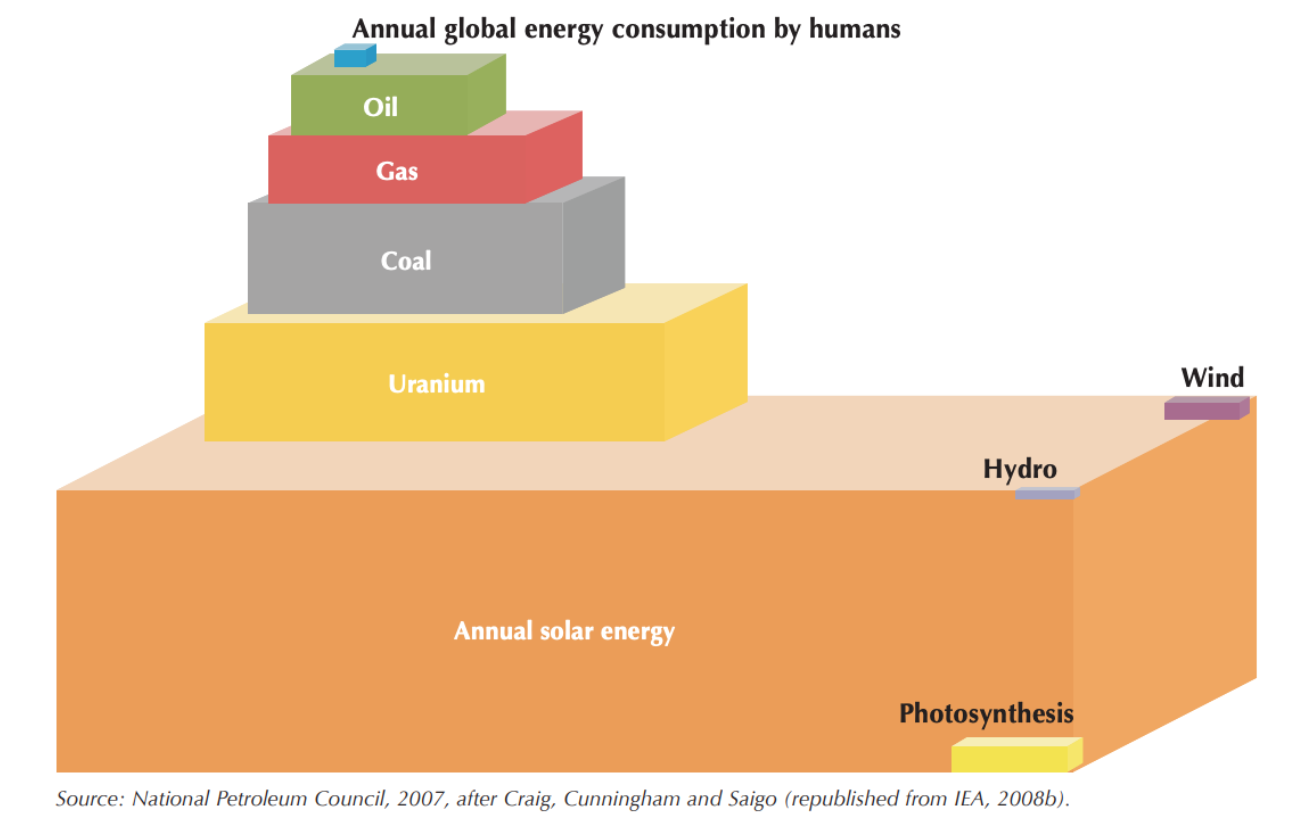
\includegraphics[width=1.0\textwidth]{power_generation_potential_sources}
	\caption[Representation of the potential energy from different sources]{Representation of the potential energy from different sources.}
	\labfig{power_generation_potential_sources}
\end{figure}

It is consequently tempting to think that it is a simple matter of capturing it. But that capture is everything but simple.

Today, if you were to think about it quickly, or ask almost anyone in the streets, the question “What is renewable energy?”, the first two responses by far would be “solar” and “wind”. In reality, those account for a tiny fraction of the renewable energy mix, which is dominated by hydroelectricity and by the biomass. Right now, you should not really picture a solar panel or a wind turbine, but a dam or a forest, especially historically.

\section{Biomass}

Biomass energy is limited by the deforestation rate. In other words, in order for the biomass energy to be considered renewable, one must not deplete the forests at a higher rate than photosynthesis replenish them.

\section{Solar}

Direct heating from sun irradiance through windows is a big natural use. Having houses that are able to do that is important, but retrofitting is not really an option. Solar heating of air or water can also be a use of solar energy, notably for showers or house flooring. Finally, the electrical conversion through photovoltaic panels can be done.


\section{Wind}

\blindtext

\section{Hydroelectricity}

\blindtext

\section{Geothermal}

\blindtext
\setchapterpreamble[u]{\margintoc}
\chapter{Nuclear}
\labch{nuclear}

In this chapter I will explain what nuclear is, and approach the main issues mentioned today, from the Thorium saver misconception to the waste problem and the safety.


\blindtext


\section{The Digest}


\begin{kaoboxgreen}[frametitle=Main Takeaways]

\begin{itemize}
\item This has not been done yet
\item Reading this will teach you absolutely nothing
\item I am serious, I could type random letters and it would give you as much information
\item Fedhiz gavartz hedtz inewps
\end{itemize}
  
\end{kaoboxgreen}
\setchapterpreamble[u]{\margintoc}
\chapter{Carbon Capture}
\labch{carbon_capture}

In this chapter I discuss carbon capture, at the source and from the atmosphere.


\blindtext


\section{The Digest}


\begin{kaoboxgreen}[frametitle=Main Takeaways]

\begin{itemize}
\item This has not been done yet
\item Reading this will teach you absolutely nothing
\item I am serious, I could type random letters and it would give you as much information
\item Fedhiz gavartz hedtz inewps
\end{itemize}
  
\end{kaoboxgreen}
\setchapterpreamble[u]{\margintoc}
\chapter{Energy Storage}
\labch{energy_storage}

In this chapter I discuss several energy storage technologies.

\begin{itemize}
\item Batteries (various kind)
\item Pumped Storage
\item Compressed Air
\item Hydrogen
\end{itemize}

Here, we discuss the importance and characteristics of energy storage, round trip efficiency, what that means, and where and what is installed in the world today (vast majority pumped storage).

\blindtext

\section{Batteries}

\blindtext

\section{Pumped Storage}

\blindtext

\section{Compressed Air}

\blindtext

\section{Hydrogen}

\blindtext


\section{The Digest}


\begin{kaoboxgreen}[frametitle=Main Takeaways]

\begin{itemize}
\item This has not been done yet
\item Reading this will teach you absolutely nothing
\item I am serious, I could type random letters and it would give you as much information
\item Fedhiz gavartz hedtz inewps
\end{itemize}
  
\end{kaoboxgreen}
\setchapterpreamble[u]{\margintoc}
\chapter{Electrical Transmission Grid}
\labch{grid}

In this chapter I talk about the grid


\pagelayout{wide} % No margins
\addpart{Climate Change, the biggest challenge in human history}
\pagelayout{margin} % Restore margins

\setchapterpreamble[u]{\margintoc}
\chapter{Greenhouse Effect, a reminder}
\labch{greenhouse_effect}

In this chapter I explain the basics of greenhouse effect.
\setchapterpreamble[u]{\margintoc}
\chapter{Climate Models}
\labch{climate_models}

In this chapter I explain the basic of CO2 emissions consequences and the climate models.


\blindtext


\section{The Digest}


\begin{kaoboxgreen}[frametitle=Main Takeaways]

\begin{itemize}
\item This has not been done yet
\item Reading this will teach you absolutely nothing
\item I am serious, I could type random letters and it would give you as much information
\item Fedhiz gavartz hedtz inewps
\end{itemize}
  
\end{kaoboxgreen}
\setchapterpreamble[u]{\margintoc}
\chapter{Natural Hazards Amplification}
\labch{natural_hazards}

In this chapter I show what people can expect, and where things are likely to get bad. 


\blindtext


\section{The Digest}


\begin{kaoboxgreen}[frametitle=Main Takeaways]

\begin{itemize}
\item This has not been done yet
\item Reading this will teach you absolutely nothing
\item I am serious, I could type random letters and it would give you as much information
\item Fedhiz gavartz hedtz inewps
\end{itemize}
  
\end{kaoboxgreen}


\pagelayout{wide} % No margins
\addpart{Transition Scenarios and Technology Costs}
\pagelayout{margin} % Restore margins

\setchapterpreamble[u]{\margintoc}
\chapter{Technology Costs}
\labch{technology_costs}

In this chapter I will go over estimating the technology costs, per unit of energy installed and produced, for the low carbon options and their necessary ancillaries\sidenote[][*7]{We will come back to that, but there is debate on the "low" part of "low carbon" for some of the technologies}. 

\begin{kaobox}[frametitle=Low Carbon Energies]
As a reminder, those low carbon energies are:

\begin{itemize}
	\item Wind
	\item Solar
	\item Water
	\item Nuclear
	\item Biomass
	\item Geothermal
\end{itemize}

Storage is the necessary ancillary for 100\% non-controllable renewable scenarios.

\end{kaobox}


Technology costs can be difficult to account for fully. For example, renewable energy, due to their decentralized nature and their high output variability, require significant, and often considered separately, transmission grid upgrades. As we will discuss, storage becomes prevalent in 100\% Renewable scenarios. And finally, the costs vary a lot by location, even within a single country, and over short periods of time.

A cost can be expressed in \$, but also in terms of our end goal, emission curtailment. We will also give a value of grams of equivalent $\mathrm{CO_2}$ per production unit for each technology.

\section{Nuclear}

Nuclear costs data varies a lot by country, depending on the workforce, the red tape, the NIMBYsm (Not In My Backyard) delays, the political will, and other considerations. Some projects are utter failures, while other seem quite successful. Hinkley Point C Power Plant, in the UK, is predicted to be four times more expensive than the identical Taishan Power Plant in China\sidenote[][-2mm]{It is an important point that we will have to consider later on. This demonstrates less a nuclear problem and more a loss of competence at building large ambitious projects}.

The prices are obtained for advanced nuclear reactors as well as small modular reactors from the EIA. 

We see that the capital cost is estimated at around \$6,100 per kW for both systems. The cost of dismantling a reactor is estimated to be between \$600 and \$1,500 per kW\sidenote[][-2mm]{In France, EDF is estimating the cost at \$350 per kW. Maybe, maybe not. I would not bet on it. At the same time, the UK is estimating the cost at up to \$3,200 per kW. Again, maybe, maybe not. And again, I would not bet on it}. Historically, hazardous waste industrial facilities dismantlement in different industries has been shown to cost around 10\% of the capital cost, which validates our estimated range further despite the lack of actual data points. A value of \$1,000 per kW of dismantlement will be used. Keep in mind that this cost is not as big as one would think in the grand scheme of transition, and that even tripling it would not impact the conclusions we will get at.

The lifetime of a nuclear plant can be taken as 60 years. It typically ranges from 40 to 80 years, with 40 years being very pessimistic, and 80 years requiring significant upgrades over the years.


\section{Gas with Carbon Capture}

\blindtext


\section{Solar}

We use the research from the National Renewable Energy Laboratory (NREL) for the cost of photovoltaic storage data. They also compute the cost of a photovoltaic and storage combined installation, but we will for now ignore those results, as we will want to account for those separately at a grid level (Feldman, 2021).


\begin{figure}[hb]
	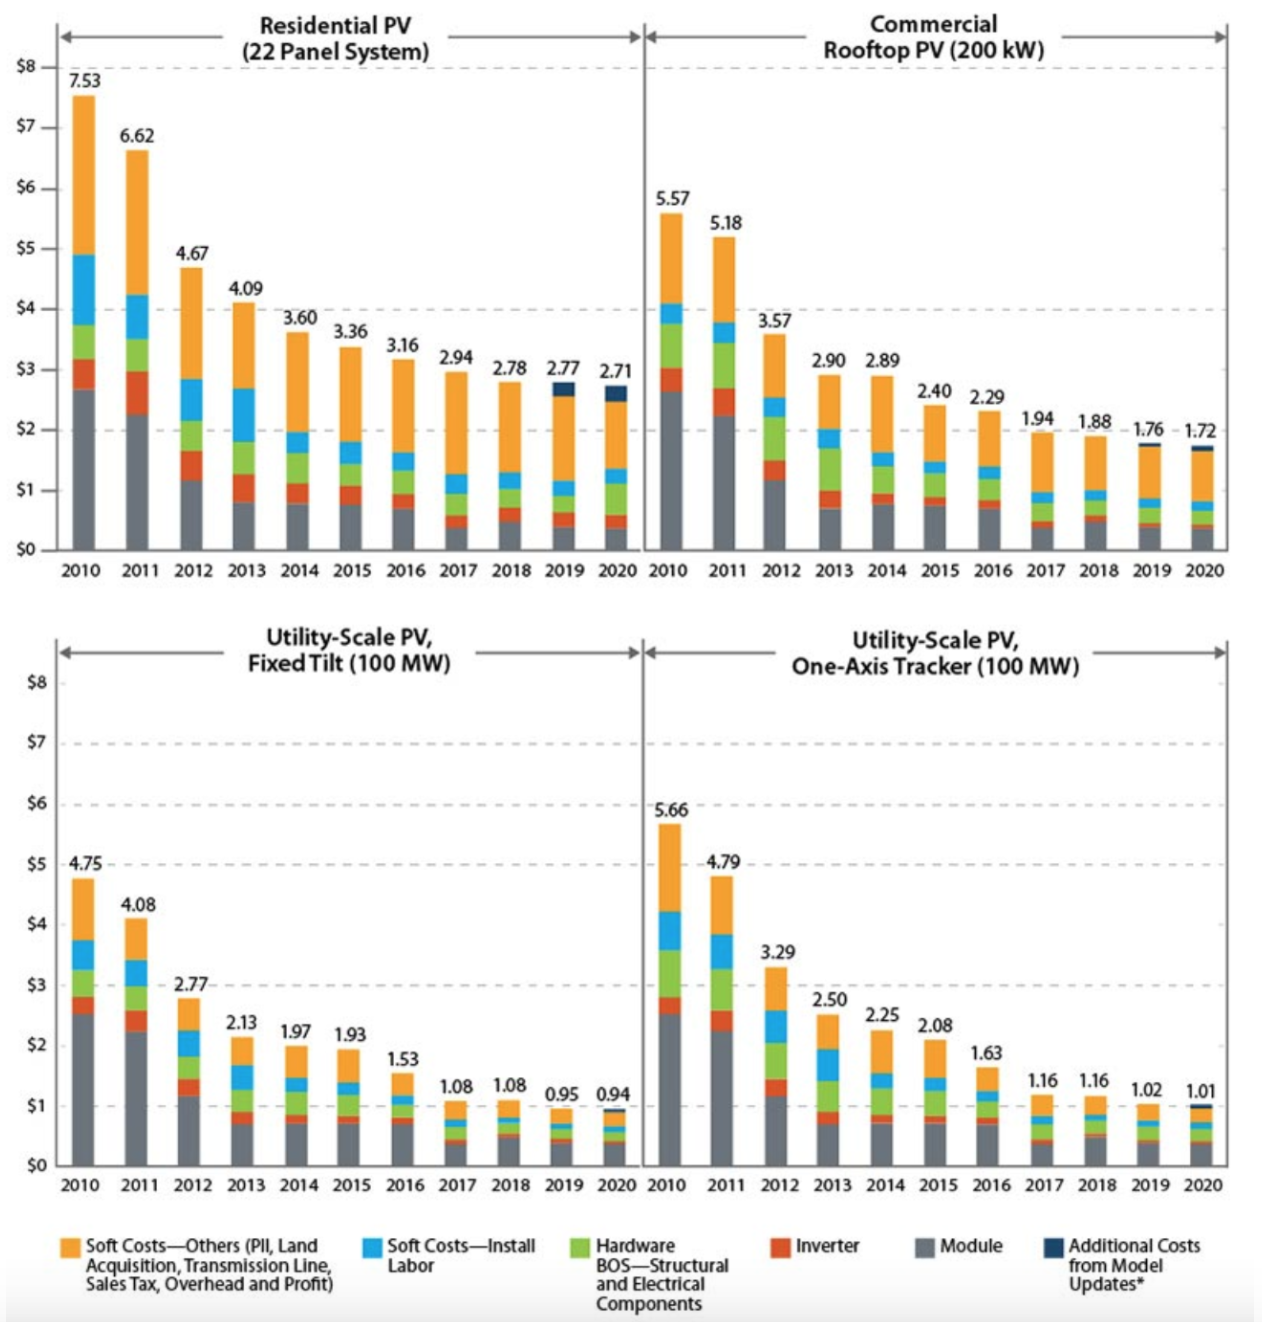
\includegraphics[width=1.0\textwidth]{solar_costs_evolution}
	\caption[Evolution of photovoltaic costs over the last decade, for several system sizes (\$/W)]{Evolution of photovoltaic costs over the last decade, for several system sizes (\$/W).}
	\labfig{solar_costs_evolution}
\end{figure}

What \vreffig{solar_costs_evolution} shows is that while the cost of installing a solar panel went down significantly over the past decades, most of the easy optimization has been done and the rate of price reduction is quickly decreasing, showing an exponential trend\sidenote[][-2mm]{In my experience, this is often glossed over in the media by simply saying that the prices for solar keep going down. Technically true, I will admit that, but nuance is always important}.

We can note that utility scale is separated into two main categories, a fixed tilt (your panel does not move) and a one-axis tracker (your panel follows the sun). The gain in load factor of the latter category is often offset by the cost difference. In this study, we will focus on the fixed tilt, while keeping in mind that a few optimizations could be done, without changing the overall conclusions.

So, what we can conclude from \vreffig{solar_costs_evolution} is that, indeed, the costs of solar energy have plummeted even in the last decade. However, we are reaching a limit that will be difficult to break through.

Consequently, in this calculation, we will assume that the current price of solar (remember, it is location dependent) is \$940 per kW, and that we can only realistically expect few gains over the next decades.


\begin{marginfigure}[-2mm]
	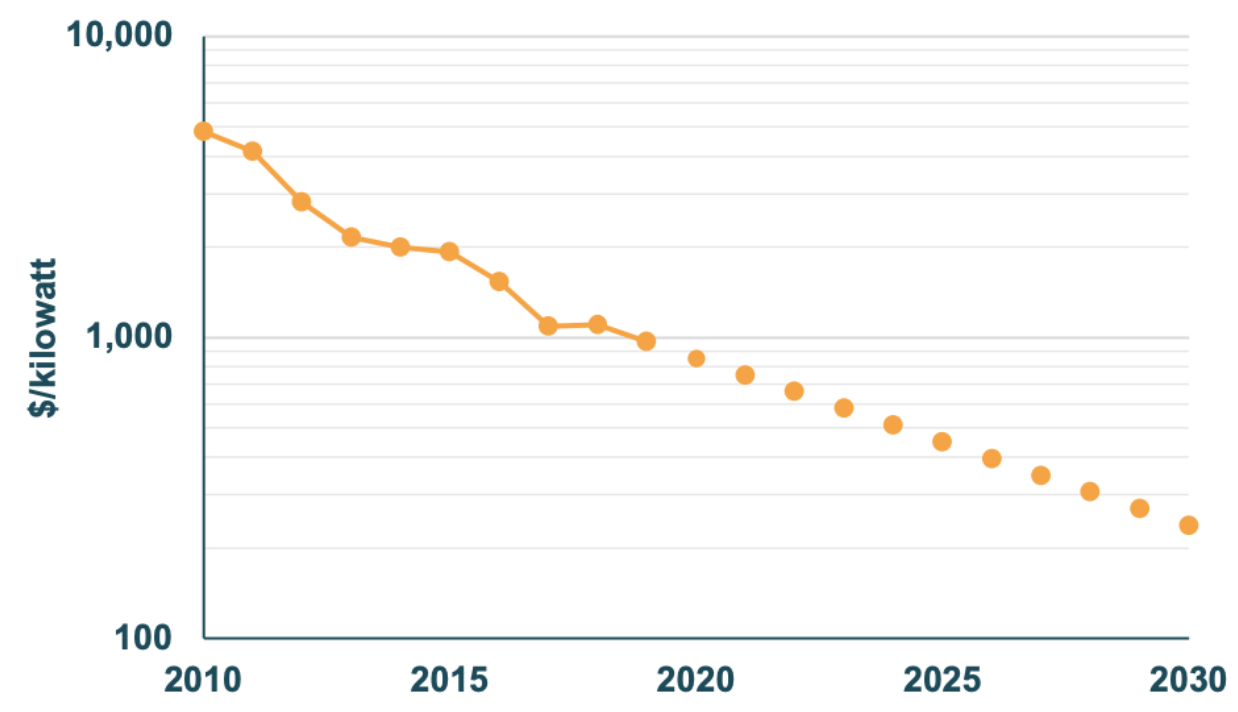
\includegraphics{dorr_optimistic_solar_costs}
	\caption[An interestingly optimistic view of the future... Solar energy manufacturing, installation and maintenance will be absolutely free before the end of the century according to some. A good reminder to be careful with your extrapolations, and the use of logarithmic scales]{An interestingly optimistic view of the future...\\ Solar energy manufacturing, installation and maintenance will be absolutely free before the end of the century according to some. A good reminder to be careful with your extrapolations, and the use of logarithmic scales.}
	\labfig{dorr_optimistic_solar_costs}
\end{marginfigure}

The lifetime of a solar installation is around 25 years. Of course, it does not fail exactly at 25 years. But degradation rates are a non negligible issues, so even if it lasts a bit longer, the gains are not enormous. We can tweak this value to test the sensitivity later on.


\section{Wind}

The wind costs have not been falling as sharply as solar in recent years. As can be seen in an NREL report on 2019 costs, onshore wind turbines will set you back around \$1,436 per kW, and offshore wind turbines around \$4,077 per kW (Stehly, 2020). It is indeed a lot more complicated to build and maintain an offshore turbine, due to the harsh ocean environment. There is a clear upside to that though, as the wind is more constant and drastically increases the load factor.

The lifetime of a wind turbine is around 25 years, give or take a few, and a little less for an offshore wind turbine, due to the harsher conditions.



\begin{figure}[hb]
	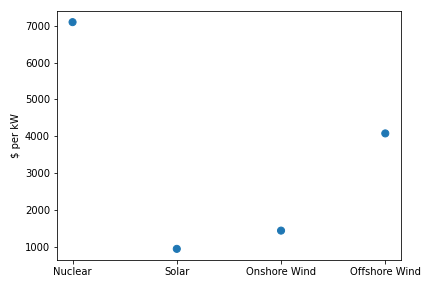
\includegraphics[width=1.0\textwidth]{technology_costs}
	\caption[2020 capital costs estimate to install various technologies]{2020 capital costs estimate to install various technologies.}
	\labfig{technology_costs}
\end{figure}


\vreffig{technology_costs} shows a damning picture for nuclear doesn't it? It is simply too expensive, several times the cost of solar and onshore wind, and even offshore wind project would be way cheaper. This is what most people, from media to politics, base their financial estimates on. And it is technically true.

But, and you knew a "but" was coming, this is misleading. Why is it misleading? Two main reasons:


\begin{itemize}
	\item Lifetime
	\item Controllable energy
\end{itemize}

A nuclear power plant has a much longer lifetime than a renewable plant\sidenote[][-2mm]{Except hydroelectricity!}. Even though, per kW, your cost is way cheaper, you do need to install several times as many kW over a long enough period of time.

On top of this, nuclear energy is a controllable energy. You turn down the dial, you have less power. You turn it up, you have more power. Solar and Wind are non controllable energy sources. We do not decide when the sun will shine or when the wind will blow. Interestingly, with the sun, we have a pretty good idea of the production times, as we know for a fact that no energy will be output at night. But cloud cover varies (fast) and we are simply not able to model it currently, and probably never will. Wind has a higher load factor, as seen previously, but the variations are quite important and unpredictable.


\begin{kaobox}[frametitle=Controllable versus Non Controllable]
A controllable energy is an energy that you control. You can decide how much power you will output and (relatively) quickly adapt to the demand consumption quick changes.

A non controllable energy is an energy that you do not control. If it's sunny, you have some, and the amount you get depends on how sunny it is, not on a button you turn. If it's not sunny, you are out of luck and must wait until the sun (or the wind) comes back to turn your TV back on. 
\end{kaobox}


\marginnote[-1cm]{There is one thing that I would like to point out, and here is as good a place as any. The low (and falling) cost of manufacturing of solar panels and wind turbines is, in part, due to easy and cheap energy sources for industrial activities, provided by fossil fuels. While I am not quantifying that value, it is not that far-fetched to see that removing that access may impact the manufacturing costs negatively, especially during a transition phase.}

What this means is that one cannot simply compare the cost of nuclear energy with the cost of solar or wind energies, as the metrics are not measuring the same things. It is the same units, \$ per kW, but the respective kW are two very different things depending on their ability to be controlled.



\begin{kaobox}[frametitle=Levelized Cost Of Electricity]
You will sometimes see the term LCOE, which stands for Levelized Cost of Electricity. What this metric does is account for time in the comparison, so that the lifetime discrepancy is corrected for.

A lot of people takes the LCOE at face value, and argue that it is the value to consider. In the current energy mix, this is correct. However, the controllability difference is still not considered, and at high enough penetration of renewable (and any 100\% renewable scenario), this does not hold true anymore from a purely physical point of view. You can install as many solar panels as you want, when it's night time, you get zero power, which you cannot afford in modern society.
\end{kaobox}


\section{Storage}

Now, we have seen the cost of installing solar and wind energy. Is that enough? Well, if we consider a 100\% Renewable scenario, we need a way to efficiently dispatch electricity to cover the varying demand.


As mentioned previously, we are going to make an assumption that I am convinced you will tend to agree with. We do want a cleaner world\sidenote[][-2mm]{We actually need it}, but we still want Netflix, we still want a choice of clothes, we still want our phones, we still want our burgers, we still want to turn on the lights whenever we want to, we still want to be able to take the train or the car to go places,\ldots In short, we still want a world at least similar to the one we are living in today. Sure, we can and will likely have to make some sacrifices and be more aware of what we can do on a day to day basis, be mindful of when to do the laundry or turn on the oven. But comfort is not going away without a fight. Additionally, I personally hope the impoverished of the world\sidenote[][-2mm]{The ones who will be disproportionately affected by climate change, remember\ldots} will have access to a better life and rise to a level of comfort at least somewhat similar to us today, which means access to energy.

So, assuming this, and accounting for a 100\% renewable energy world, it is easy to see that to meet our needs, the means of production will have to become controllable. This is where energy storage comes into play.

We will consider multiple options, from the proven pumped storage stations to the highly hyped battery energy storage system\sidenote[][-2mm]{Often simply called “batteries” or “grid-scale batteries” in the news articles you may have come across}. Pacific Northwest National Laboratories (PNNL) data will be used as reference. Interestingly, they give a value in 2018 as well as an estimated projection up to 2025. In this report, we will consider the more advantageous 2025 values given (Mongird, 2019).

For a battery energy storage system, out of the multiple options available (Sodium-Sulfur, Li-Ion, Lead Acid, Redox Flow, \ldots), the cheapest is selected, that is Li-Ion, at \$1,446  per kW and \$362 per kWh. The lifetime of such batteries is 10 years, maybe 15 years could be doable by 2025.

\begin{kaobox}[frametitle=Energy storage: kW versus kWh]
Recall the energy storage section for the difference between the cost per kW (power capacity, what you can store) and the cost per kWh (energy capacity, what you can get back)
\end{kaobox}


Let’s now look at the more classical options, namely pumped storage stations (PHS) and below-ground compressed air energy storage (CAES). According to the same PNNL report, pumped storage clocks in at a cost of \$2,638 per kW and \$165 per kWh, while compressed air storage is given at around \$1,669 per kW and \$105 per kWh. The lifetime of a pumped storage station has been estimated to be around a century, while a compressed air storage system is given at 25 years.

While compressed air storage is cheaper, the conversion ratio, or in other words the losses incurred by the storage and restitution of the energy is much lower.

Consequently, we will for now consider the best storage technology on the long term, which is the pumped storage hydroelectric solution. It is coincidentally the only one that has really been used at a non-negligible scale and for a long time. We will come back to the other technologies later on.


\section{Grid}

The grid network is very often overlooked. It is now a cost that is folded into an energy source technology, despite the fact that it depends strongly on what energy is being used.

Those costs are extremely difficult to project, especially for a 100\% renewable system for which no data point exists. Studies (IER, 2019) have shown a cost roughly a third of the investment in the production means themselves (solar panels, wind turbines). However, countries currently developing it, such as Germany, have seen an actual cost impact on production of 100\%. In other words, 1 dollar spent on the installed renewable capacity required another dollar invested onto the grid infrastructure.

In this study, we will consider the value above of one-third of the investments made, which correspond to roughly \$500 per kW renewable installed. A sensitivity analysis will also be performed to see the impact of modifying this parameter.


\blindtext


\section{The Digest}



\begin{table*}[h]
\caption[2020 technology costs estimates]{2020 technology costs estimates}
\labtab{technology_costs_estimates}
\begin{tabular}{ c c c c }
	\toprule
	Technology & Capacity Installation & Storage Installation & Grid upgrades \\
	\midrule
	Nuclear & \$7,100 per kW (25y) & Not Applicable & Not Applicable\\
	Solar & \$950 per kW (25y) & \$165 per kWh (100y) & \$500 per kW (50y)\\
	Onshore Wind & \$1,436 per kW (25y) & \$165 per kWh (100y) & \$500 per kW (50y)\\
	Offshore Wind & \$4,077 per kW (25y) & \$165 per kWh (100y) & \$500 per kW (50y)\\
	\bottomrule
\end{tabular}

\end{table*}

\begin{kaoboxgreen}[frametitle=Main Takeaways]

\begin{itemize}
\item The costs for multiple technologies were obtained from reputable sources.
\item Be mindful of extrapolating cost data into the future. You will get it wrong, the question is by how much.
\item System lifetime matters, and LCOE is not an adequate measure depending on the context. 
\item Storage is very expensive.
\end{itemize}
  
\end{kaoboxgreen}



\setchapterpreamble[u]{\margintoc}
\chapter{Carbon Footprints}
\labch{carbon_footprints}

In this chapter I will go over estimating the carbon footprints for each technology.



\section{Direct versus Indirect emissions}

Fossil fuels emit a lot of carbon equivalent gases into the atmosphere. For several generation sources, often referred to as "clean", there is no direct greenhouse gases emissions. This is the case for nuclear, wind, solar, geothermal, biomass and hydroelectricity. However, this does not mean that these technologies do not have a carbon footprint. Indeed, the intensive manufacturing process of the capture elements (wind turbines, solar panels, reactor buildings, \ldots) emit a non negligible amount of $\mathrm{CO_2}$. These emissions are denoted "indirect".

When discussing installed capacity and energy produced, it is important to consider the load factors, or capacity factors. These measures represent how often one generates the optimal output from a technology. In other words, say you have a power plant with a capacity of 1 GW. THis means that in theory, you could get 8760 GWh of energy out of it. But if it's off 50\% of the time, and operating at 75\% of its power for the rest of time, you will only get 3285 GWh out, or 37.5\% of the theoretical maximum. THe capacity factor of your plant is then 37.5\%. While some load factors are artificially reduced\sidenote[][*-1]{Nuclear and thermal power plants suffer in part from having to follow the load, and in part due to a market effect}, some are physically limited\sidenote[][*2]{Wind, Solar, and Hydroelectric generate power only when the wind is blowing, the sun is shining, and sufficient water level is in a reservoir}. France proves to be a good benchmark for a real world case study of nuclear at a large scale, as the lower load factor (in the 60-70\% range, compared to values in the 90\% neighborhood for countries such as the USA, as we will see later) demonstrates the ability of nuclear energy to “load-follow”. On the other hand, production of electricity from solar and wind installed capacity is cheap and even close to free\sidenote[][*1]{Solar and wind indeed do not have any fuel cost, though they do have some maintenance costs}, so a lower value here would be dictated almost entirely by physical limitations in the current market-driven grid.


\begin{kaobox}[frametitle=Load Follow]
Load-Following is the act of quickly adapting the production to the demand by ramping up or down the output of the power plant.
\end{kaobox}

\begin{kaobox}[frametitle=A look at some values]

Let us take a step back and consider how the emissions are usually scored. You will see values given in $gCO_2/kWh$. This is a value one has to be careful with, as a kWh may not be representative of an indirect emission. Solar is usually cited at around 50 g per kWh.

To illustrate this, consider two 5kW solar systems, both built in the exact same way, same plant, same location. Then, use one of these systems in Fairbanks, AK, and the other in Phoenix, AZ. As expected, the performance would be radically different, and we can for example assume the load factor to be 10\% in Fairbanks and 30\% in Phoenix. In that situation, the Alaskan system would generate 4,400 kWh, while the Arizonian system would generate 3 times as much, at 13,000 kWh, over a year.

So, this implies that the Alaskan solar system emits 220 kilograms of $\mathrm{CO_2}$
per year and the Arizonian solar system emits 650 kilograms of $\mathrm{CO_2}$ (still the factor 3).

But this is obviously incorrect, as the emission from solar are indirect, and thus both system emitted the same amount of $\mathrm{CO_2}$, when they were manufactured.

In order to compute the right value, the $gCO_2/kWh$ should be accompanied by a capacity factor value or at least a location, or in other words, the $gCO_2/kW$ should be given.

This issue is true of every means of production where the emissions are indirect and occur during manufacturing.

\end{kaobox}

\begin{figure}[h]
	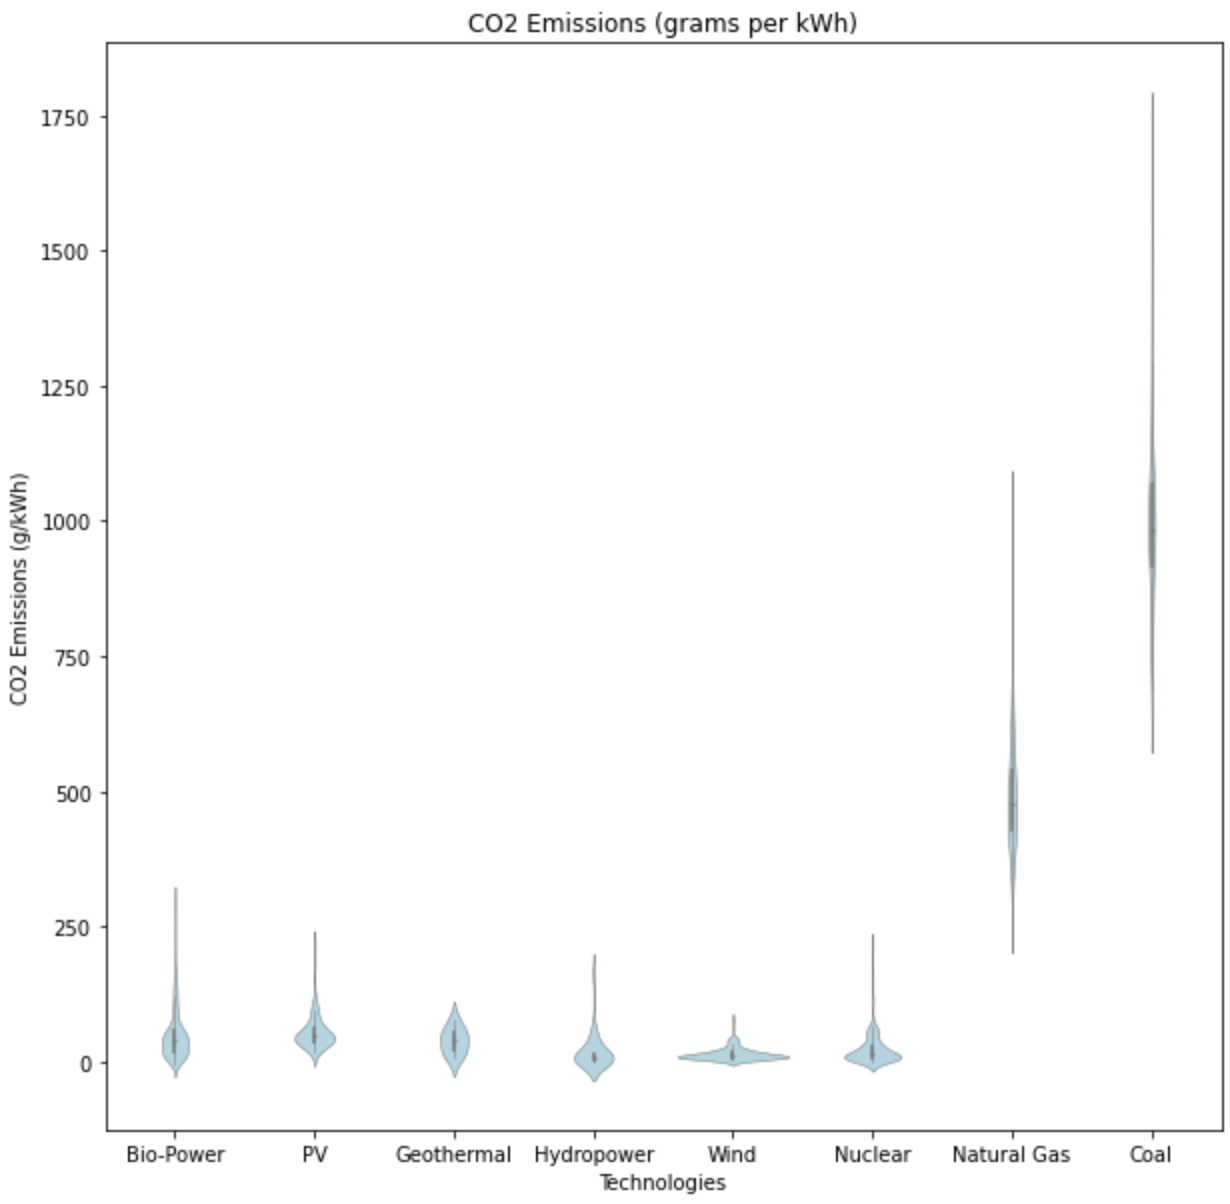
\includegraphics[width=1.0\textwidth]{co2_tech}
	\caption[Adjusted $\mathrm{CO_2}$ Emissions per technology. Keep in mind that this is dependent on capacity factors for the indirect carbon emissions.]{Adjusted $\mathrm{CO_2}$ Emissions per technology. Keep in mind that this is dependent on capacity factors for the indirect carbon emissions.}
	\labfig{co2_tech}
\end{figure}



\section{Technologies footprint}

%SOLAR
%https://www.nature.com/articles/ncomms13728
% In SI, Table 2, we get the CO2 per kW
The indirect $\mathrm{CO_2}$ emissions of solar energy has been shown to be around 1 kg per Wp in the last decade~\sidecite{louwen2016re}. This translates to 1 ton per kWp installed. Another way to think about this is that the manufacturing and installation of your average residential solar roof generates around 5 tons of $\mathrm{CO_2}$. These initial emissions are offset in a few years, depending on the energy mix where the panels are producing.

Wind data is a bit lacking in terms of indirect emissions. Values are often given per location, without explicitly mentioning the assumptions made. We will thus estimate the carbon footprint from harmonized $gCO_2/kWh$ median values\sidecite{dolan2012life}. \vreffig{co2_solar_wind} shows the $\mathrm{CO_2}$ cost for both solar and wind.


\begin{figure}[h]
	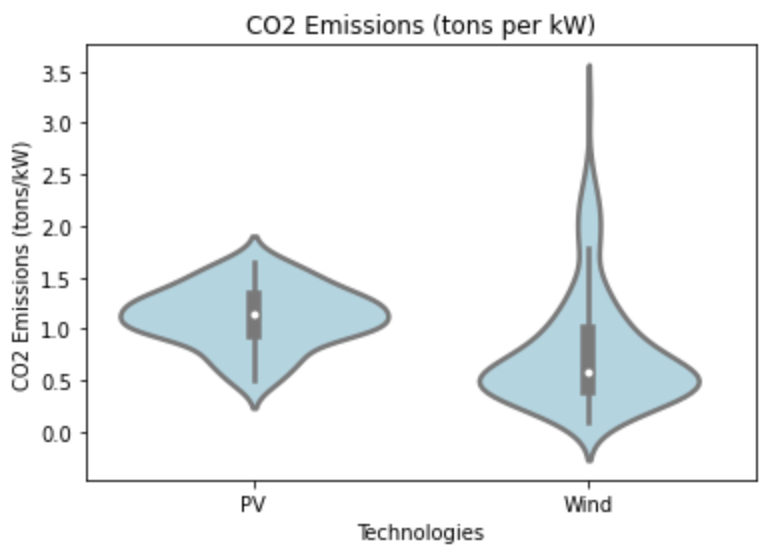
\includegraphics[width=1.0\textwidth]{co2_solar_wind}
	\caption[Adjusted $\mathrm{CO_2}$ Emissions (indirect) for solar and wind power, assuming 30\% capacity factor and 20 years lifetime for wind, and 15\% capacity factor with a 30 years lifetime and a degradation rate of 0.7\% per year for solar.]{Adjusted $\mathrm{CO_2}$ Emissions (indirect) for solar and wind power, assuming 30\% capacity factor and 20 years lifetime for wind, and 15\% capacity factor with a 30 years lifetime and a degradation rate of 0.7\% per year for solar.}
	\labfig{co2_solar_wind}
\end{figure}

An average system of 1 kW installed capacity (capacity factor 30\%, lifetime 20 years) will generate $8760h * 20y * 30\% = 52.5 MWh$. At $11 gCO_2/kWh$, this represents around 0.6 ton of $\mathrm{CO_2}$ per kW.

The batteries impacts in terms of $\mathrm{CO_2}$ emissions are difficult to estimate. To get a reasonable order of magnitude, we use data from~\sidecite{dai2019life,emilsson2019lithium}, and assume a energy mix closer to the Chinese one, where the majority of the battery production happens today. This gives us around 100 kg of $\mathrm{CO_2}$ per kWh capacity installed\sidenote[][]{Note that when it comes to batteries, kWh capacity is not kWh produced, due to the lifetime (number of cycles)}.

Nuclear emissions have been shown to be around a median of 17 $gCO_2/kWh$~\sidecite{warner2012life}. Using the relevant capacity factor of 92\%, and an operational lifetime of 40 years, we can see that each kW of nuclear installed comes with a cost of carbon of approximately 
5 tons per kW, as shown by the median value on~\vreffig{co2_nuclear}. One can note that at first glance, it might seem that nuclear generates 5 to 10 times more $\mathrm{CO_2}$. Be mindful, and recall that our goal here is to get a development carbon cost, meaning that we decorrelate the lifetime and capacity factor (to generate the same energy over time, you need to install a lot more kW of renewable)\sidenote[][-2mm]{Do not compare indirect $gCO_2/kW$ values without care}.

\begin{figure}[h]
	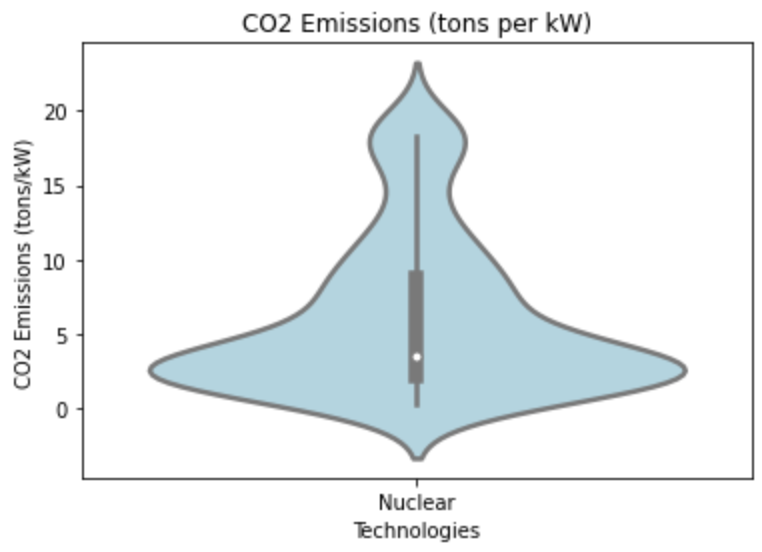
\includegraphics[width=1.0\textwidth]{co2_nuclear}
	\caption[$\mathrm{CO_2}$ Emissions (indirect) for nuclear power.]{$\mathrm{CO_2}$ Emissions (indirect) for nuclear power, assuming a 92\% capacity factor. We can see some high values, resulting from worst case scenarios on the ore type and the enrichment method notably.}
	\labfig{co2_nuclear}
\end{figure}

Natural gas, Coal and Petroleum are clear emitter at production (direct emissions). From the literature, we see that we can approximate natural gas emissions at 475 $gCO_2/kWh$ produced~\sidecite{o2014life}. Coal shows large variability depending on the technology, but a value of 1,000 $gCO_2/kWh$ produced is a good approximation~\sidecite{whitaker2012life}.


\begin{figure}[h]
	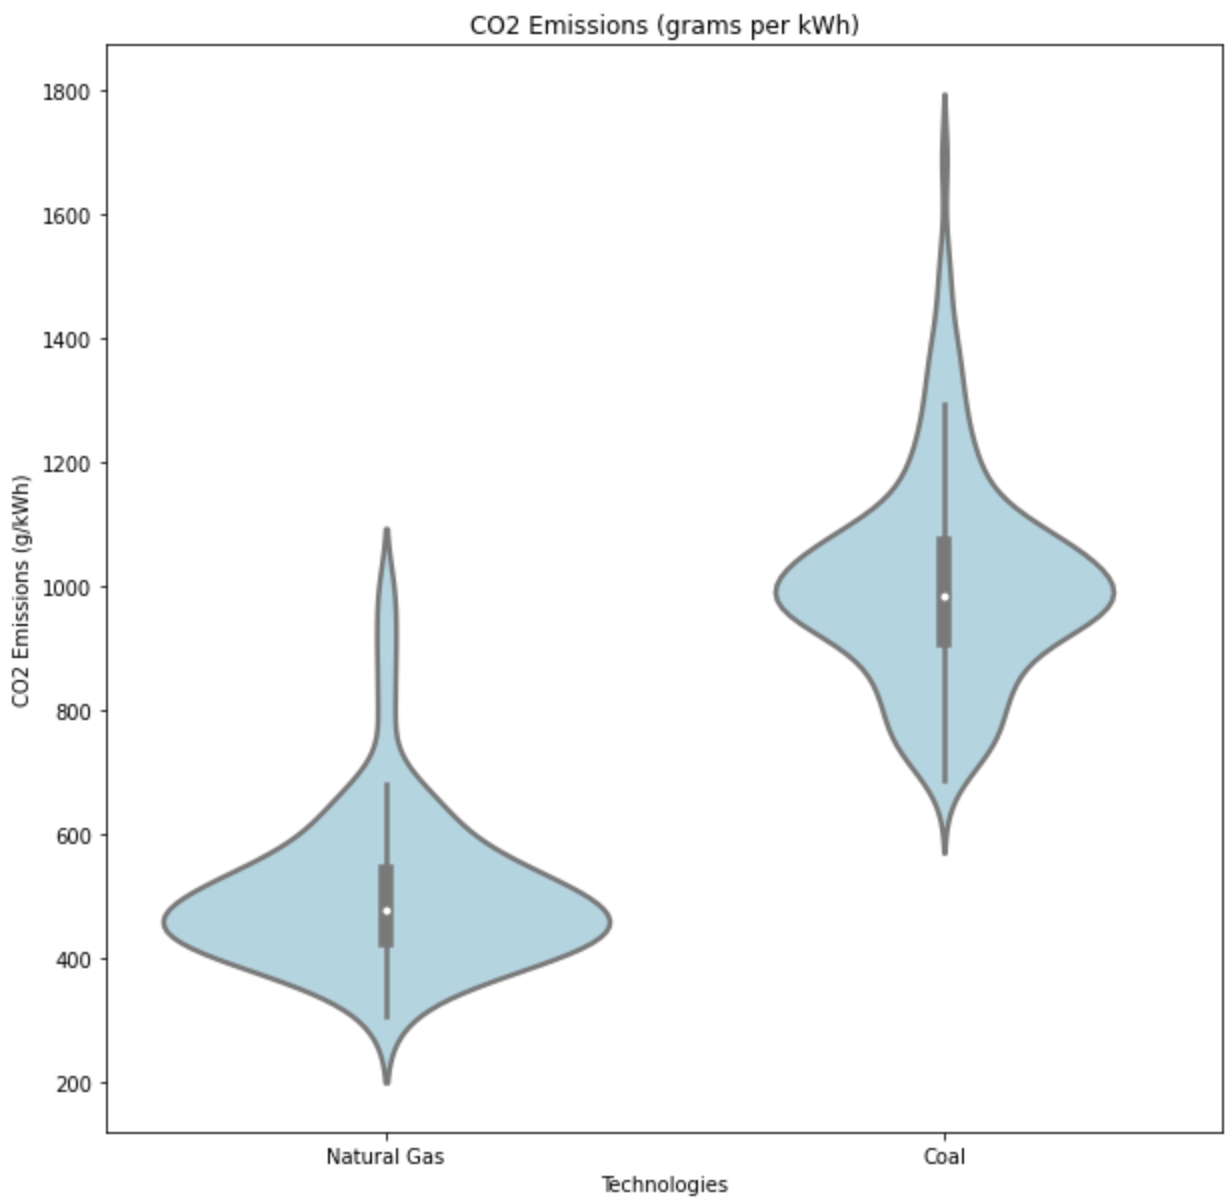
\includegraphics[width=1.0\textwidth]{co2_coal_gas}
	\caption[$\mathrm{CO_2}$ Emissions (direct) for coal and gas power.]{$\mathrm{CO_2}$ Emissions (direct) for coal and gas power.}
	\labfig{co2_coal_gas}
\end{figure}


\begin{kaobox}[frametitle=Indirect emissions\ldots until a cleaner grid?]

It is also important to note that the reason why the indirect emissions of renewable energies manufacturing is so high is due to the current energy mix of the manufacturing places. A solar panel made in China will have a higher $\mathrm{CO_2}$ cost than a solar panel made in Europe, because of the type of energy used in its manufacturing.

As the grid moves toward a cleaner version, the indirect emissions will decrease. At the same time, it is easy to think that the more the grid moves toward a cleaner version, the more the cost and ease of mining and manufacturing could go up.

\end{kaobox}


\begin{table}[ht]
\caption[Carbon emissions per technology]{Carbon emissions per technology}
\labtab{carbon_emissions_technology}
\begin{tabular}{ c c c }
	\toprule
	Technology & Direct (g/kWh) & Indirect (tons/kW) \\
	\midrule
	Natural Gas & 475 & - \\
	Coal & 1000 & - \\
	Nuclear & - & 5000 \\
	Petroleum & 1000 & - \\
	Solar & - & 1 \\
	Wind & - & 0.6 \\
	Hydro & 15 & - \\
	Batteries & - & 100\sidenote[*][-2mm]{kg per kWh capacity} \\
	\bottomrule
\end{tabular}

\end{table}


\section{The Digest}

\begin{kaoboxgreen}[frametitle=Main Takeaways]

\begin{itemize}
\item Normalized by energy produced over their lifetime in an average environment, Nuclear and the renewable energies (Hydroelectricity, Biomass, Solar and Wind) are comparable in terms of emissions, and much lower than fossil fuels.
\item The distinction direct versus indirect emissions is important, as theoretically, almost all indirect emissions could be removed given a clean energy grid.
\item Clean energy emits $\mathrm{CO_2}$ during the manufacturing process, which requires energy from the existing grid, and thus the use of fossil fuel in most cases.
\item Chemical batteries are a non-negligible emitter due to their energy intensive mining and manufacturing process in today's grid. On the other hand, pumped hydro storage has a low carbon footprint.
\end{itemize}
  
\end{kaoboxgreen}


\todo{Appendix: How to read a violin plot?}

\setchapterpreamble[u]{\margintoc}
\chapter{Transition Scenarios}
\labch{transition_scenarios}

We will assume four main categories of transition scenarios for each country as a first-order approximation.

\begin{itemize}
	\item \textbf{S1:} 100\% single renewable technology scenarios
	\item \textbf{S2:} 100\% multiple renewable technologies scenarios
	\item \textbf{S3:} 100\% Nuclear scenarios
	\item \textbf{S4:} Mix of nuclear with multiple renewable technologies scenarios
\end{itemize}

\todo{Appendix Or Chapter: What about\ldots ? Gravity towers, Hydrogen, Ocean Waves, Fusion} 

The Nuclear Scenario replaces and expands the nuclear program in the countries where it exists to cover 100\% of the electrical demand, and create one where it does not. The 100\% single renewable scenario phases out both fossil fuels and nuclear energy from the electricity and energy generation mix, and replaces them with one technology\sidenote[][-2mm]{Only onshore wind power, or only solar power, for example}. Of course, those scenarios are an exaggeration of what the near future may look like, but it will still be interesting to compare their respective viability. No scenarios involving fossil fuels for electricity generation are acceptable, as the end goal is to transition to low carbon energy sources. The 100\% multiple renewable scenario takes this a step further by allowing the renewable mix to be accounted for. And finally, we show what the impact of a mix of nuclear and renewable could look like.

We will not consider exports or imports of electricity, as we assume that the neighbors encounter similar issues in their transitions, and energy independence is considered an important factor. Note that this assumption is valid when considering the first order impact of our scenarios. Geopolitics make it so that full cooperation with high dependence for something as critical as the energy infrastructure is not something nations will accept readily, even between strong allies. We also assume that electricity consumption stays constant over time, but that energy needs decreases with an electrical basis.

Additionally, and importantly, the main assumption is that we want a world and a society that is not radically different from today, hence the ability to dispatch energy when and where you want it.

Another crucial point we consider is that the low-carbon grid we want needs to be sustainable. It is not enough to switch to a low carbon system and, once its lifetime is up, give up on it. Lifetime cycles need to be accounted for over a long period. In this demonstration, we consider 100 years to be a representative period. We will drop this to 50 years to see the sensitivity.

\begin{kaobox}[frametitle=The total transition cost is X Trillions\ldots]
You may come across articles or headlines that claim that the cost of transition to a fully decarbonized system is a given amount of trillions of dollars for a given country. This does not have to be false, but, again, we want a sustainable, long term grid. If we had a technology today that was able to completely decarbonize our grid for \$5 trillion dollars for a country like the USA and could be built in a month, it would be great, nay, incredible. But if I then told you that the lifetime of that technology is one year, so that every year, you needed to rebuild it anew, the cost would be incredibly high and crippling to the current world economy. Even if this was doable, it would then go against the assumption that we do not want to change to a radically different society in a very short time span. In my experience, this is ignored most of the time, and is coherent with the easy pitfalls of "this is the next-generation problems" tropes that we have seen in recent history.
\end{kaobox}



Again, recall that we want only a simplistic first-order comparison. Our goal is not to build a complex model, optimized and tuned to decades of historical and projected data\sidenote[][-2mm]{Those models are set in an ideal Utopian world where crisis are non-existent and society is more stable than any other time in history. I am rooting for this, but I like to stay reasonable}. We aim to show what one can reasonably expect from various scenarios and draw conclusions from this. Policies have never been made on complex, perfectly optimized simulations. If the first order calculation does not agree with a complex model, it does not mean the complex model is wrong per se, but that its implementation is unlikely to work as intended, because humans are not always rational actors unfortunately.

\section{Scenarios S1}

We define the S1 scenarios as being the 100\% single renewable energy scenarios. This implies that for each scenario in this category, the entire energy generation fleet is driven by one technology. This is of course an implausible assumption, but one that will allow us to derive useful information nonetheless.

\begin{kaobox}[frametitle=S1 scenarios]
\begin{itemize}
	\item \textbf{S1a:} 100\% Wind (onshore) coupled with Pumped Hydroelectric Storage
	\item \textbf{S1b:} 100\% Wind (onshore) coupled with Batteries Storage
	\item \textbf{S1c:} 100\% Wind (offshore) coupled with Pumped Hydroelectric Storage
	\item \textbf{S1d:} 100\% Wind (offshore) coupled with Batteries Storage
	\item \textbf{S1e:} 100\% Solar coupled with Pumped Hydroelectric Storage
	\item \textbf{S1f:} 100\% Solar coupled with Batteries Storage scenarios
\end{itemize}
\end{kaobox}

By its nature, a grid composed of 100\% renewable resources is not viable to deliver a society similar to what we are all used to currently, and what I'm fairly certain we all wish for the future\sidenote[][-2mm]{This does not mean no consumption adaptation, it simply means we are looking to lower the bar of necessary changes to let it be realistic}. We will use the two most prevalent technologies in the discussions, pumped hydroelectricity storage and batteries. So, exactly how much storage do we need?

To answer this question, the first thing we need to know is:

\begin{itemize}
\item What is the maximum period of time where our needs could be unmet?
\end{itemize}

An important thing to note here is that when we say that the needs are not meet, it does not mean that we get no power from our installed capacity. It means that we do not get enough power from our installed capacity. Ten days of wind production at 20\% is equivalent to two days of no wind at all.

Common scenarios are a gloomy week, or a sustained storm. In those cases, solar and wind production will be hampered. It is not unreasonable, and pretty accepted, to think that 7 days of storage would be needed. Keep in mind that if you do not have enough storage in place and run out, the whole economy stops. We will modify the duration to test the sensitivity to storage need, from 1 to 7 days.


\begin{remark}
The energy to store is given by~\ref{energy_store}, $t$ varying between 1 and 7 days (it has to be given in number of hours).

\begin{equation}\label{energy_store}
E_s = t * \frac{E_a}{8760}
\end{equation}

\end{remark}

Round-trip efficiency represent the fraction of the electricity that you put in that you can expect to get back. Indeed, you will not get back everything you sent to your storage, due to cable losses, inverter or mechanical losses, and various other factors. This efficiency is variable between technologies and over time. A good approximation is between 65\% and 85\%\sidenote[][-2mm]{As an example, for pumped storage, the main sources of losses are approximately 5\% to the network itself, 80\% to the pumping stations and 85\% to the turbines, which translates to 65\%, and thus a loss to storage of 35\%.}. 

This has a strong implications. In order to get back the energy you would need, you have to send $\frac{1}{0.85} = 1.18$ to $\frac{1}{0.65} = 1.55$ times as much electricity. This has a potential impact on the capacity that has to be installed to begin with.

We will assume that this does not matter for our first order calculation, and that we have enough power generation to fill in sufficient storage power capacity by default. Additionally, we consider that the extra power generated when demand is low can be easily curtailed or used in alternate, non-time sensitive process. This encompasses hydrogen production or desalination, for example, two energy intensive processes\sidenote[][-2mm]{Energy is only one of the drivers of these processes challenges.}.

All the scenarios discussed will consider the existing grid, decommission what needs to be decommissioned, and rebuild everything from scratch to a 100\% technology penetration for a period of 100 years.

For simplicity sake, we do not consider the currently installed capacity of the given production technology. This does not impact the results, given the scale and timeframe of the transitions.


\section{Scenarios S2}

Obviously, the one-generating-technology scenarios are on the extreme, unrealistic side. The load factor considered in a renewable mix will be more advantageous due to a combination effect\sidenote[][-2mm]{You can have wind when you do not have solar, and vice versa. But keep in mind that the limiting factor will often be windless or low-wind nights, which are not uncommon, and which you need to plan for with storage}.

In those scenarios, we will play with the type of renewable mix we develop during the transition, by changing the ratio of solar versus wind power notably.


\begin{kaobox}[frametitle=S2 scenarios]
\begin{itemize}
	\item \textbf{S2a:} 50\% Wind (75\% onshore and 25\% offshore), 50\% Solar, coupled with pumped hydroelectric storage
	\item \textbf{S2b:} 50\% Wind (75\% onshore and 25\% offshore), 50\% Solar, coupled with batteries storage
	\item \textbf{S2c:} 30\% Wind (75\% onshore and 25\% offshore), 70\% Solar, coupled with pumped hydroelectric storage
	\item \textbf{S2d:} 40\% Wind (75\% onshore and 25\% offshore), 70\% Solar, coupled with batteries storage
	\item \textbf{S2e:} 70\% Wind (75\% onshore and 25\% offshore), 30\% Solar, coupled with pumped hydroelectric storage
	\item \textbf{S2f:} 70\% Wind (75\% onshore and 25\% offshore), 30\% Solar, coupled with batteries storage
\end{itemize}
\end{kaobox}

We chose those shares in each scenario, but keep in mind that it can be modified at will, and that we can account for a mix of the storage technologies too. Storage need will be impacted by a renewable mix, as they would be able to compensate the weaknesses of one another up to a point.


%We have seen an approximation, which we will use for our simplified scenarios S1 through S6\todo{Improve this part. We can maybe remove the production hours graphs and simply assume that we need to meet consumption assumption an X day period to compensate for. We need to show how a mix impacts the storage needs by combining hourly data from both wind and solar over a period. The question is thus to find hourly data for solar production in a given year and combine it with hourly data for wind production in the same year and same location, to compute the storage requirements}. Let's see how we can factor in a more realistic system, where a mix of renewable energies is used, with wind, solar and hydro working in unison over larger areas.

The first thing we need to know is:

\begin{itemize}
\item Given a mix of renewable energies, what is the maximum period of time where our needs are not met?
\end{itemize}

This will vary depending on the mix you define.


\begin{figure}[ht]
	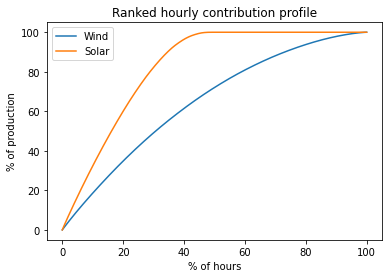
\includegraphics[width=1.0\textwidth]{renewable_production_hours_ranked}
	\caption[Percent of hours in a year contributing to a percent of the output, ranked by importance]{Percent of hours in a year contributing to a percent of the output, ranked by importance.}
	\labfig{renewable_production_hours_ranked}
\end{figure}

The \vreffig{renewable_production_hours_ranked} may be a bit difficult to read, so let me spend some time explaining what went on here. In order to generate this plot, I used one year of hourly power output for both wind and solar power. The solar data was simulated over Texas using synthetic solar photovoltaic from NREL. The wind data was downloaded from the ERCOT website, the Texan grid operator. This data consequently approximates potential redistribution of power generation between different part of the state of Texas.

Knowing the power generated every hour of the year, I then ranked them from most productive to least productive. So, if you take the solar data for example, the "noons" of the year are first, and the nightly hours come later, not contributing any power to the production. From that, I then plotted where each hour falls in the year ranking against the percentage of production.

In other words, what this graph shows is that for solar power, once you reach the 40\% of the top contributing hours, you have generated all the yearly power. The remaining 60\% do not contribute power. This is logical, as it is night 50\% of the time and your panels are more efficient in direct sunlight than in the evening, when it gets hit only by diffuse sunlight.

Another way of interpreting this graph is that 80\% of solar power production is done in only 30\% of the time during the year, leaving you at risk of not meeting production demand the rest of the time because you can easily find period where multiple consecutive hours are in those 70\% remaining hours.

Wind is less predictable, but has more contributing hours during a year. You do not have a clear cycle like nights and days, and it varies a bit more regionally than the sun irradiance. 80\% of the production from wind power comes from 60\% of the time, leaving you at risk during 40\%. Using this data, what we can conclude as a first order approximation is that your needs, with solar, would be covered 30\% of the time, while they would be covered 60\% of the time for wind\sidenote[][-2mm]{A complex model can give better results there, by combining the solar or wind data with an estimation of the hourly load notably, at the risk of over-optimization leading to a less resilient grid and more frequent blackouts. Our approach is still a pretty good first order approximation of the scale we are talking about.}.

Consequently, we can say that in the most favorable situation, wind would cover for solar at night, and wind is low only during the day.

\begin{remark}
In that case, based on a reasonable 80\% of the total production being viable:

\begin{itemize}
\item It's sunny enough for 30\% of the time, and not windy enough for 40\% of the time
\item It's windy enough for 60\% of the time, and not sunny enough for 70\% of the time
\end{itemize}

So, on first order approximation, we can say that 10\% of the energy need cannot be met, even under the most ideal, fairy tale scenario.

\end{remark}

One can consider adding hydroelectricity or geothermal to the mix and think that this could meet 100\% of the demands and to not have a storage requirements~\sidecite{hoste2009matching,brown2018synergies}. It has however been shown to be reliant on assumptions that are on the very optimistic side~\sidecite{boretti2020cost,clack2017evaluation}, notably because of short term strong variability. A different way to look at it is that it may work for larger regions with strong interconnections and links, such as the European Union and the United States of America, and in a beautifully engineered infrastructure which would have to be flawless\sidenote[][-2mm]{From a purely geopolitical and national security perspective, it is not far-fetched to consider the impact on balance of power at small and abrupt time scale.}.

%In this section, we will consider the short term unpredictable variability of solar and wind, and consider that even only 10\% of the energy needs have to come from storage\sidenote[][*6]{Keep in mind that while this is theoretically possible, it is physically unlikely to be the case. That's the limitation with theoretical models, they tend to assume that everything works a bit too much as expected}.


\begin{remark}

In this renewable energy mix scenario, which does imply an important paradigm shift in society consumption and grid operation to add leniency, the amount of storage needed consequently is given by~\ref{energy_store}, $t$ varying between 1 and 7 days and becomes:

\begin{equation}\label{energy_store}
E_s = f_s * t * \frac{E_a}{8760}
\end{equation}

Here, we assume, as seen previously, that an optimist assumption for the fraction of energy to store is $f_s = 10\%$.


\end{remark}


\section{Scenarios S3}

The S3 scenarios are made up of only one scenario, a 100\% nuclear grid. In order to get to this, we will first get rid of all the existing installed capacity, with the associated dismantling costs, and rebuild everything from scratch to cover the entirety of a country electricity needs.

Nuclear has shown that it can follow loads on short time scale. While some may disagree that a 100\% nuclear could function efficiently due to this issue, it is still a reasonable assumption to make.


\begin{kaobox}[frametitle=S3 scenarios]
\begin{itemize}
	\item \textbf{S3a:} 100\% Nuclear
\end{itemize}
\end{kaobox}


\section{Scenarios S4}

The nuclear and renewable mix is a scenario in which a given share of the energy production is driven by nuclear energy, while the rest is produced by renewables.

This presents, as will be demonstrated later on, a clear advantages in that it does not require large, grid-scale storage capabilities. It can answer to multiple concerns about all the scenarios S1, S2, and S3.

We vary the share of nuclear versus renewable energies to show the impact of a nuclear-heavy energy production as well as a renewable heavy production.


\begin{kaobox}[frametitle=S4 scenarios]
\begin{itemize}
	\item \textbf{S4a:} 50\% Nuclear, 50\% Renewables (30\% Wind onshore, 10\% Wind offshore and 60\% Solar)
	\item \textbf{S4b:} 50\% Nuclear, 50\% Renewables (40\% Wind onshore, 20\% Wind offshore and 40\% Solar)
	\item \textbf{S4c:} 25\% Nuclear, 75\% Renewables (30\% Wind onshore, 10\% Wind offshore and 60\% Solar)
	\item \textbf{S4d:} 25\% Nuclear, 75\% Renewables (40\% Wind onshore, 20\% Wind offshore and 40\% Solar)
	\item \textbf{S4e:} 75\% Nuclear, 25\% Renewables (30\% Wind onshore, 10\% Wind offshore and 60\% Solar)
	\item \textbf{S4f:} 75\% Nuclear, 25\% Renewables (40\% Wind onshore, 20\% Wind offshore and 40\% Solar)
\end{itemize}
\end{kaobox}





\section{The Digest}


\begin{kaoboxgreen}[frametitle=Main Takeaways]

\begin{itemize}
\item We define four main categories of scenarios, from all renewable to all nuclear, with some mixes.
\item Each categories is divided into a given number of scenarios where some parameters are modified.
\item Nineteen scenarios are computed to be representative of the potential options considered.
\end{itemize}
  
\end{kaoboxgreen}



















%Multiple scenarios will be tested from the two categories we defined.


%\begin{kaobox}[frametitle=Scenarios to consider]

%\begin{itemize}
%	\item S1: Onshore Wind -- Pumped Hydro Storage
%	\item S2: Onshore Wind -- Batteries
%\item S3: Offshore Wind -- Pumped Hydro Storage
%	\item S4: Offshore Wind -- Batteries
%	\item S5: Solar -- Pumped Hydro Storage
%	\item S6: Solar -- Batteries
%	\item S7: Nuclear
%	\item S8\footnote{We can vary the share of each technologies. By default, we use 30\% onshore wind, 10\% offshore wind,  60\% solar mix, and 50\% batteries, 50\% pumped storage}: Renewable Mix -- Storage Mix
%	\item S9\footnote{We can vary the share of each technologies. By default, we use 24\% wind onshore, 8\% wind offshore, 48\% solar, 20\% nuclear mix}: Nuclear -- Renewable Mix
%\end{itemize}

%Each of the scenarios will furthermore be tested for sensitivity by modifying parameters and looking at a range of future potentials, from pessimistic to optimistic depending on the energy source.

%\end{kaobox}



\pagelayout{wide} % No margins
\addpart{First Order System Assessments}
\pagelayout{margin} % Restore margins

\setchapterpreamble[u]{\margintoc}
\chapter{The Transition Needs}
\labch{transition_needs}

In this chapter I will assess two main scenarios. The first one assumes that the world of 2050 and later looks very similar to the world of today. That is, energy poverty, and by extension poverty, is not solved and the needs do not increase. We even look at an optimistic energy need, where the fossil fuels heat conversion is replaced by a more effective use of electricity, lowering the energy needs. A second scenario is also shown where we consider everyone on the planet to have a reasonable access to energy, with every country consuming at the Eastern European rate.

\begin{kaobox}[frametitle=Transition Scenarios]
\begin{itemize}
\item Scenario EOSP

The scenario Energy Optimist, Society Pessimist consider that the current energy needs only are transitioned. This means that the billions of people currently in energy poverty stay in that position for the next century.

\item Scenario EPSO

The scenario Energy Pessimist, Society Optimist consider that the world will see the electrification of most people living in poverty today, at a level  around 30,000 kWh or energy consumed per year per capita. As a reference point, this is roughly the situation of Poland, Greece or Portugal.
\end{itemize}
\end{kaobox}

Scenario EOSP indicates the need to transition 160,000 TWh, while scenario EPSO would have us transition 200,000 TWh.


\todo{Clarify GWe versus GWth}


When the media discuss energy transition, I feel that they often misrepresent, or don't explain enough, what they mean. There is a very large difference between electricity and energy. Electricity encompasses only the electric power uses, such as what allows a home outlet to charge a phone, plug a fridge, etc. Energy consists of all of the electricity as well as transportation and heating.

When using gas to power a car or to heat a location, a lot of the energy is lost in the process. Electricity would allow you to be more efficient. Consequently, the electrification of the transportation and thermal sector implies a better efficiency and less consumption, translating to a lower power needed.

In the following, we will make two things distinct:


\begin{kaobox}[frametitle=Electricity Transition]
Electricity transition is the removal of all energy from fossil fuels from the electrical grid. In other words, the gasoline powered cars can stay, the coal and gas plants have to go.
\end{kaobox}

\begin{kaobox}[frametitle=Energy Transition]
Energy transition is the removal of all energy from fossil fuels, to be replaced with non carbon-emitting sources.
\end{kaobox}

Electricity transition is not energy transition.


\section{Current Energy Sources}

The data for the current energy generation mix in the world is obtained.

[Placeholder for energy donut graph]

[Placeholder for energy time series graph]

[Placeholder for zoom on renewable share graph]




Energy use:

Primary energy includes heat conversion. The IEA gives estimates of the total final consumption~\sidecite{iea2020statistics}, in millions of tons of oil equivalent (MTOE). In an all electric world, this is what matters. From that, let's try and see what cannot be transitioned for now.

The fossil fuels consumption to replace is consequently 1000 MTOE for coal, 4000 MTOE of Oil, and 1500 MTOE of Natural Gas. Coal is used at 30\% for iron and steel production, at 10\% for petrochemical uses, and 20\% for non-metallic minerals, with another 5\% for non-energy use. The transition pathways for those applications seem difficult to achieve soon. The rest of the coal consumption, roughly 35\%, could be transitioned. Oil is used for industrial consumption (plastics notably) and for non-energy applications such as lubricants and other products. We can assume that 75\% of the energy consumed from oil could be transitioned, notably from the transportation sector. 12\% of natural gas is used for non-energy purposes, and we can approximate that 85\% could be transitioned to clean energy.

%Coal: 1000 MTOE
%--> 30\% iron and steel
%--> 10\% petrochemical
%--> 20\% non-metallic minerals
%--> 5\% non-energy use
%--> Rest (35\%) could transition

%Oil: 4000 MTOE
%--> 16\% non energy (lubricants etc)
%--> 8\% industrial (plastics etc)
%--> Rest (75\%) could transition

%Gas: 1500 MTOE
%--> 12\% non energy
%--> Rest (85\%) could transition

So, we could transition around $0.35 * 1000 + 0.75 * 4000 + 0.85 * 1500 = 4625 MTOE$. This represents 70\% of the fossil fuels consumption today. Note that fossil fuels account for around 70\% of the total energy consumption themselves.

%0.35 * 1070 + 0.75 * 3985 + 0.85 * 1502 = 4640 out of 6557 MTOE, or 70%

%In 2017, fossil fuels accounted for 6557 MTOE out of 9717 MTOE, or around 70\%


The world today uses ~160,000 TWh of equivalent primary energy. It breaks down, roughly to:

\begin{itemize}
\item Oil: 55,000 TWh (primary)
\item Natural Gas: 40,000 TWh (primary)
\item Coal: 45,000 TWh (primary)
\item Nuclear: 7,000 TWh (electricity)
\item Hydro: 10,000 TWh (electricity)
\item Renewable: 8,000 TWh (electricity)
\end{itemize}

In the case of fossil fuels, we see that the primary energy consumed is given. This is due to the fact that there is a penalty to using heat engine, as it's not a very efficient process, and approximately two third of the primary energy is lost in the process of converting to electricity. We want to assess the needs in a 100\% electrified world. This means that we can get rid of the heat efficiency issue for fossil fuels notably and replace with a more efficient electricity use.

We have seen above that we can imagine replacing around 70\% of our fossil fuels needs with electricity. This represents around 100,000 TWh, distributed across three main sectors: transportation, electricity, and direct heat. No change in energy consumption is to be expected from the direct heat sector, and renewables will have trouble making a dent in that sector. It consists mostly of industrial processes requiring very high temperatures. Biomass or waste fuels could be used, but could encounter a not-renewable-anymore issue.

Transportation represents around a third of the fossil fuel use. The efficiency of a modern gasoline car is around 30\%. The efficiency of an EV is around 75\%. In order to replace all the gasoline used in transportation, we need to replace approximately 50,000 TWh of fossil fuel (oil). If our EVs were 100\% efficient at converting electricity to power, we would need 30\% of the 50,000 TWh, or 15,000 TWh. Since they are around 75\% efficient, our actual need is 15,000 TWh divided by 75\%, or 20,000 TWh\sidenote[][-2mm]{This represents a heat rate conversion factor of 40\%. You may find that number when people compare primary energy between fossil fuels and renewables.}. Consequently, if the entire transportation sector were to switch to electric vehicles, the energy requirements would drop from 50,000 TWh to 20,000 TWh, or by 60\%.

Electricity represents around another third of the fossil fuels uses. For the power plants part, we can assume a relatively similar heat rate to convert. We do have a higher efficiency in a turbine than in a gasoline car, but we also have a higher efficiency of our renewable energy production system than batteries trips. Here we want to transition approximately 50,000 TWh again. So we get, using our 40\% efficiency conversion factor, a drop in our energy requirements from 50,000 TWh to 20,000 TWh again, or another 60\% drop.


From these first order estimates, we conclude that maximizing the electrification of the energy grid would mean that we go from around 160,000 TWh to 100,000 TWh, or a 35 to 40\% drop, all else being equal (EOSP scenario). In the EPSO scenario, the needs would increase, and consequently we would have to meet 130,000 TWh via electricity.


It's important to note that those estimates are very optimistic, both in terms of actual transition feasibility and in terms of future energy needs. It assumes the transition of the entire world transportation sector (so, not one gasoline powered car left), and of most things that can technically transition to an electricity source.

%Assuming an extremely optimistic electrification of the world transport sectors and other heat engines, let us assume that only 150000 TWh of energy will be needed every year. Note that this is probably on the very, very low end of future needs.

\section{Current Carbon Emissions}

This section computes an estimate of the yearly carbon emissions in both scenarios assuming a business-as-usual situation. This will give us a good idea of what we need to avoid producing.


\section{Scenarios Pathway}

This section looks at all the installation we need for each scenario. It should be a table:



\begin{table}[ht]
\caption[Technology capacity per Scenario S1]{Technology capacity per Scenario S1}
\labtab{technology_capacity_scenarios_s1}
\begin{tabular}{ c c c c c c c }
	\toprule
	Technologies & S1a & S1b & S1c & S1d & S1e & S1f \\
	\midrule
	Solar & - & - & - & - & - & - \\
	Offshore Wind & - & - & - & - & - & - \\
	Onshore Wind & - & - & - & - & - & - \\
	Conventional Nuclear & - & - & - & - & - & - \\
	Advanced Nuclear & - & - & - & - & - & - \\
	Small Modular Nuclear & - & - & - & - & - & - \\
	Batteries & - & - & - & - & - & - \\
	Pumped storage & - & - & - & - & - & - \\
	\bottomrule
\end{tabular}
\end{table}


\begin{table}[ht]
\caption[Technology capacity per Scenario S2]{Technology capacity per Scenario S2}
\labtab{technology_capacity_scenarios_s2}
\begin{tabular}{ c c c c c c c }
	\toprule
	Technologies & S2a & S2b & S2c & S2d & S2e & S2f \\
	\midrule
	Solar & - & - & - & - & - & - \\
	Offshore Wind & - & - & - & - & - & - \\
	Onshore Wind & - & - & - & - & - & - \\
	Conventional Nuclear & - & - & - & - & - & - \\
	Advanced Nuclear & - & - & - & - & - & - \\
	Small Modular Nuclear & - & - & - & - & - & - \\
	Batteries & - & - & - & - & - & - \\
	Pumped storage & - & - & - & - & - & - \\
	\bottomrule
\end{tabular}
\end{table}


\begin{table}[ht]
\caption[Technology capacity per Scenario S3]{Technology capacity per Scenario S3}
\labtab{technology_capacity_scenarios_s3}
\begin{tabular}{ c c c c c c c c c }
	\toprule
	Technologies & S3a & S3b & S3c \\
	\midrule
	Solar & - & - & -  \\
	Offshore Wind & - & - & -  \\
	Onshore Wind & - & - & -  \\
	Conventional Nuclear & - & - & -  \\
	Advanced Nuclear & - & - & -  \\
	Small Modular Nuclear & - & - & -  \\
	Batteries & - & - & -  \\
	Pumped storage & - & - & -  \\
	\bottomrule
\end{tabular}
\end{table}

\begin{table}[ht]
\caption[Technology capacity per Scenario S4]{Technology capacity per Scenario S4}
\labtab{technology_capacity_scenarios_s4}
\begin{tabular}{ c c c c c c c }
	\toprule
	Technologies & S4a & S4b & S4c & S4d & S4e & S4f \\
	\midrule
	Solar & - & - & - & - & - & - \\
	Offshore Wind & - & - & - & - & - & - \\
	Onshore Wind & - & - & - & - & - & - \\
	Conventional Nuclear & - & - & - & - & - & - \\
	Advanced Nuclear & - & - & - & - & - & - \\
	Small Modular Nuclear & - & - & - & - & - & - \\
	Batteries & - & - & - & - & - & - \\
	Pumped storage & - & - & - & - & - & - \\
	\bottomrule
\end{tabular}
\end{table}

\section{The Digest}


\begin{kaoboxgreen}[frametitle=Main Takeaways]

\begin{itemize}
\item The world consumes today around 160,000 TWh of energy, mostly from fossil fuels
\item Electrifying the world is a goal we should all have in mind. This implies increasing the energy consumption to around 200,000 TWh.
\item Electrification of the transport and heating sector would save primary energy, and we can imagine that this would drop the requirements by around one third.
\end{itemize}
  
\end{kaoboxgreen}
\setchapterpreamble[u]{\margintoc}
\chapter{Scenarios Case Study}
\labch{scenario_computation}

In this chapter I will go over computing the amount of capacity to install, the amount of storage to install, the impact to expect on the grid, and the impact of a renewable mix versus what we will end up computing, a homogeneous system.



\section{Recalling the Assumptions}

The question of electricity imports and global exchange is important, and a difficult one to account for. That is, if there is not enough electricity available in France, can I ask my neighbors to sell me some? In our first order calculation, we are considering that no, this is not an option. The reasoning why follows. Say you have a dark, cold, calm day in France. Your wind and solar energies sources are thus severely hampered. You technically would have three options.

\begin{itemize}
	\item Use your storage capacity
	\item Ask the neighbors
	\item Learn to not use electricity
\end{itemize}


Well, from multiple observations in Europe, when such a situation happens somewhere in France for example, things are not looking great in other parts of Europe, due to meteorological effects such as anticyclones and depressions. This is especially within immediate neighboring countries such as Germany or Spain. Any electricity the neighbors would produce would be used for their own needs, and put into their storage for future domestic use if any is left. Our main assumption is that the installed capacity is enough to power yourself, but that you are not building up out of the goodness of your heart for your neighbors\sidenote[][-2mm]{And I argue that it makes for a poor investment to try and overbuild your capacity even more to sell your surplus, as most of your surplus would happen when other countries are not especially in dire need}.

We also assume that consumption stays constant over time. Additionally, and importantly, the main assumption is that we want a world and a society that is not radically different from today, hence the ability to dispatch energy when and where you want it.

Another crucial point to consider is that the low-carbon grid we want needs to be sustainable\marginnote[-2mm]{You may come across articles or headlines that claim that the cost of transition to a fully decarbonized system is a given amount of trillions of dollars for a given country. This does not have to be false, but, again, we want a sustainable, long term grid. If we had a technology today that was able to completely decarbonize our grid for \$5 trillion dollars for a country like the USA and could be built in a month, it would be great, nay, incredible. But if I then told you that the lifetime of that technology is one year, so that every year, you needed to rebuild it anew, the cost would be incredibly high and crippling to the current world economy. Even if this was doable, it would then go against the assumption that we do not want to change to a radically different society in a very short time span. In my experience, this is ignored most of the time, and is coherent with the easy pitfalls of "this is the next-generation problems" tropes}. It is not enough to switch to a low carbon system and, once its lifetime is up, give up on it. Lifetime cycles need to be accounted for over a long period. In this demonstration, we consider 100 years to be a representative period. We will drop this to 50 years to see the sensitivity.


\begin{table}[ht]
\caption[Input Data and Notations]{Input Data and Notations}
\labtab{input_notations}
\begin{tabular}{ c c c }
	\toprule
	Data & Notation & Units\\
	\midrule
	Annual Energy Production Needs & $E_a$ & TWh \\
	Installed Capacity & $P_i$ & GW\\
	Technology Load Factor & $f$ & \% \\
	Peak Production & $p_{max}$ & \% \\
	Energy Storage Capacity & $E_s$ & TWh\\
	Power Storage Capacity & $P_s$ & GW \\
	Power Excess & $P_e$ & GW \\
	Storage Round-Trip Efficiency & $e$ & \% \\
	Installed Capacity with Storage & $P_{i,s}$ & GW \\
	Minimum Yearly Need & $P_{min}$ & GW \\
	Energy Storage Fraction & $f_s$ & \% \\
	Installation Costs & $C_i$ & \$ \\
	Storage Costs & $C_s$ & \$ \\
	Dismantling Costs & $C_d$ & \$ \\
	Grid Costs & $C_g$ & \$ \\
	Duration of Storage need & $t$ & hours \\
	\bottomrule
\end{tabular}
\end{table}


\section{How Many GigaWatts?}

We have seen from \vrefch{transition_needs} the amount of energy to be produced annually, in TWh, per country of interest. In that chapter we also derived the load factor per technology, in the latest years.


An important factor to consider now is the capacity of electricity you need to install in order to obtain this necessary energy produced at the end of any given year. This is shown in equation~\ref{eqn_power_installed}.

\begin{remark}
In order to obtain the energy generated over a year in Wh, one needs to multiply the power installed by the number of hours in a year\sidenote[][-2mm]{Mind the units! Recall that $E_a$ is in Terrawatt-hour, which is a thousand Gigawatt-hour and a billion kilowatt-hour. So, the $P_i$ obtained will be in Terrawatt. We are most used to dealing with installed capacity in Gigawatt, which implies a multiplication by $10^{-3}$ of your result}.

\begin{equation}\label{eqn_power_installed}
P_i = \frac{E_a}{f * 8760}
\end{equation}

\end{remark}

\section{Storage Requirements}



\begin{kaobox}[frametitle=What we have said]
Wind and Solar can be down or low for extended periods of time, during which batteries have to pick up the slack. This represents $x$ TWh over the year and gives us a battery output required assuming a duration period to cover of $y$ days.

While this may seem to not take advantage of a combining effect, this is actually a reasonable assumption in the real, non-perfectly-optimized, world. In such optimized modeling simulations, real world constraints such as geopolitics and social difficulties are often ignored or misrepresented.

\end{kaobox}







\section{Grid impact}

We are making the assumption here that the grid is able to deal with a lot of excess energy, or that this is used for non-time-dependent processes like hydrogen production, desalination, or other. This comes with grid requirements which can be very difficult to meet.

Grids have been designed to accommodate for around the power capacity that is currently installed, in a mostly centralized, optimized, system. In order to move to a 100\% renewable system, hence mostly decentralized, non-optimized, system, grid developments will be necessary, and transmission lines will have to be built. In terms of cost, it is no secret that it is a lot more expensive to install 500 lines of 100 MW (accommodating an installed capacity of 50 GW) than 25 lines of 2 GW (accommodating the same installed capacity). Materials, public works, distance covered, all those and more factor into the increased price.

More importantly, the installed capacity being greater, the grid has to be reinforced to account for the maximum expected output. While the load factor over the year is relatively low for wind or solar, you will have peaks throughout the year at up to 70\% and 90\% of the installed capacity respectively\sidenote[][-2mm]{A sunny day at noon, a windy day on all your wind farms, and all of the sudden you have way more energy than you know what to do with!}. 

You are presented with three basic options for this energy.
\begin{itemize}
\item Store it
\item Use it
\item Dump it
\end{itemize}

The first option is to store it for future use as long as you have the installed storage power capacity. Given your requirements, this has to be done in priority. The second option is to use that excess energy for auxiliary uses, such as hydrogen production. This is not as simple as it seems, and is unfortunately not a magical solution, though it has a lot of merits. The third option is to accept the loss and curtail your production.


\begin{remark}
Consequently, the grid should be ready to deal with an excess power up to what is given in the following equation.

\begin{equation}\label{excess_power}
P_e = P_i * p_{max} - P_{min}
\end{equation}
\end{remark}


\section{Energy Mix}

As mentioned several times, we are considering homogeneous scenarios. The production comes either from solar, or from wind, or from nuclear, and so forth. In reality, a mix would be beneficial for multiple reasons, including economical competition and load factor smoothing. Load factor smoothing would be the idea that you have nights, you have windless days, but since you have windy nights or sunny calm days, by definition the overlaps increases the load factor of your system.

We can use the simulated data discussed previously to quickly estimate the impact.

\begin{itemize}
\item Get the solar production per hour
\item Get the wind production per hour
\item Sum the two
\item Get the load factor for solar only
\item Get the load factor for wind only
\item Get the load factor for combination
\end{itemize}



\section{The Digest}


\begin{kaoboxgreen}[frametitle=Main Takeaways]

\begin{itemize}
\item We derive the main simple equation to be used to approximate the costs of a scenario
\item The capacity to install per scenario is given depending on a constant need assumption
\item The storage consequence is approached, and we go easy on it
\end{itemize}
  
\end{kaoboxgreen}
%\setchapterpreamble[u]{\margintoc}
\chapter{A Renewable Problem}
\labch{renewable_problem}

In this chapter I will go over the approximate costs incurred in each of the nine scenario we have defined, listed on the side.

We will pull the data we have described in \refch{transition_needs} and \refch{technology_costs} and apply the reasoning derived in \refch{renewable_solution}.


\begin{kaobox}[frametitle=Scenarios to consider]

\begin{itemize}
	\item S1: Onshore Wind -- Pumped Hydro Storage
	\item S2: Onshore Wind -- Batteries
	\item S3: Offshore Wind -- Pumped Hydro Storage
	\item S4: Offshore Wind -- Batteries
	\item S5: Solar -- Pumped Hydro Storage
	\item S6: Solar -- Batteries
	\item S7: Nuclear
	\item S8: Renewable Mix -- Storage Mix
	\item S9: Nuclear -- Renewable Mix
\end{itemize}

Each of the scenarios will furthermore be tested for sensitivity by modifying parameters and looking at a range of future potentials, from pessimistic to optimistic depending on the energy source.

\end{kaobox}

\section{Electricity Transitions}

First, we calculate an estimate of the costs per scenario, for each country, in \vreftab{scenario_costs_estimates}. This shows that things get very expensive, and that some options are clearly more efficient economically than others. \vreftab{scenario_costs_ratio} shows the normalization relative to the least expensive scenario each time\sidenote[][-2mm]{Nuclear, with a score of 1}. Even though in our case studies we do not vary the prices locally, and assume that a project will cost the same in every country, we see that the ratios vary. This is mostly due to the effect of changing load factors. Not every country is equal when it comes to natural resources, and wind and solar are natural resources.


\begin{table}[ht]
\caption[Scenario Costs Estimate over 100 years per country (Trillions US Dollars -- Electricity only -- 7 days of storage)]{Scenario Costs Estimate over 100 years per country (Trillions 2020 US Dollars) -- Electricity only -- 7 days of storage -- Backup Factor}
\labtab{scenario_costs_estimates}
\begin{tabular}{ c c c c c c c c c c }
	\toprule
	Country & S1 & S2 & S3 & S4 & S5 & S6 & S7 & S8 & S9 \\
	\midrule
	France & 1.9 & 9.1 & 3.2 & 8.7 & 2.7 & 17.2 & 1.2 & S8 & S9\\
	USA & 12.2 & 71.4 & 17.7 & 62.1 & 15.2 & 133.5 & 9.1 & S8 & S9\\
	Brazil & 1.4 & 9.6 & 2.4 & 8.6 & 2.2 & 18.6 & 1.2 & S8 & S9\\
	China & 29.2 & 128.8 & 40.8 & 115.5 & 31.5 & 230.8 & 15.2 & S8 & S9\\
	Nigeria & 0.08 & 0.46 & 0.11 & 0.4 & 0.09 & 0.85 & 0.06 & S8 & S9\\
	Nigeria\sidenote[$\dagger$][-2mm]{With access to an average French person electricity}  & 4.2 & 23.1 & 5.6 & 19.8 & 4.7 & 42.5 & 2.9 & S8 & S9\\
	\bottomrule
\end{tabular}
\end{table}


\begin{table}[ht]
\caption[Scenario Costs Estimate over 100 years per country (Trillions US Dollars -- Electricity only -- 7 days of storage)]{Scenario Costs Estimate over 100 years per country (Trillions 2020 US Dollars) -- Electricity only -- 7 days of storage}
\labtab{scenario_costs_estimates}
\begin{tabular}{ c c c c c c c c c c }
	\toprule
	Country & S1 & S2 & S3 & S4 & S5 & S6 & S7 & S8 & S9 \\
	\midrule
	France & 2.5 & 20.6 & 3.9 & 22.0 & 2.9 & 21.0 & 1.2 & 2.0 & 1.7\\
	USA & 12.2 & 71.4 & 17.7 & 62.1 & 15.2 & 133.5 & 9.1 & S8 & S9\\
	Brazil & 1.4 & 9.6 & 2.4 & 8.6 & 2.2 & 18.6 & 1.2 & S8 & S9\\
	China & 29.2 & 128.8 & 40.8 & 115.5 & 31.5 & 230.8 & 15.2 & S8 & S9\\
	Nigeria & 0.08 & 0.46 & 0.11 & 0.4 & 0.09 & 0.85 & 0.06 & S8 & S9\\
	Nigeria\sidenote[$\dagger$][-2mm]{With access to an average French person electricity}  & 4.2 & 23.1 & 5.6 & 19.8 & 4.7 & 42.5 & 2.9 & S8 & S9\\
	\bottomrule
\end{tabular}
\end{table}


\begin{table}[ht]
\caption[Scenario Costs Ratios Estimate over 100 years per country (Trillions US Dollars -- Electricity only -- 7 days of storage)]{Scenario Costs Ratios Estimate over 100 years per country (Trillions 2020 US Dollars) -- Electricity only -- 7 days of storage}
\labtab{scenario_costs_estimates}
\begin{tabular}{ c c c c c c c c c c }
	\toprule
	Country & S1 & S2 & S3 & S4 & S5 & S6 & S7 & S8 & S9 \\
	\midrule
France & 1.6 & 7.6 & 2.7 & 7.3 & 2.3 & 14.3 & 1 & S8 & S9\\
USA & 1.3 & 7.8 & 1.9 & 6.8 & 1.7 & 14.7 & 1 & S8 & S9\\
Brazil & 1.2 & 8.0 & 2.0 & 7.2 & 1.8 & 15.5 & 1 & S8 & S9\\
China & 1.9 & 8.5 & 2.7 & 7.6 & 2.1 & 15.2 & 1 & S8 & S9\\
Nigeria & 1.3 & 7.7 & 1.8 & 6.7 & 1.5 & 14.2 & 1 & S8 & S9\\
$\mbox{Nigeria}^{\dagger}$ & 1.4 & 8.0 & 1.9 & 6.8 & 1.6 & 14.7 & 1 & S8 & S9\\
	\bottomrule
\end{tabular}
\end{table}







%\sidenote[\dagger][-2mm]{With access to an average French person electricity} 
Another way to express it is as a ratio value. How much more expensive than the minimum cost over all considered scenario?

\blindtext


\section{Energy Transitions}

We do the same tables and figures here but for energy as a whole.


\blindtext


\section{Sensitivity Analysis}

This section models the impact of changing the prices, increasing or decreasing the demand, modifying the storage duration.

\blindtext

\section{The Digest}


\begin{kaoboxgreen}[frametitle=Main Takeaways]

\begin{itemize}
\item All the scenarios are compared in terms of absolute estimated costs and relative costs
\item The goal is not only to transition to a clean energy environment, but to transition to a long-term sustainable environment
\item Nuclear is the cheapest option when looking at a reasonable time frame, and a sensitivity analysis shows that it would take a lot of things going against markets expectations to be more cost efficient
\item Batteries are the biggest economic hurdles for renewable systems
\end{itemize}
  
\end{kaoboxgreen}




\setchapterpreamble[u]{\margintoc}
\chapter{Scenario Assessments -- Renewable}
\labch{scenario_assessments}

In this chapter I will go over the physical limitations of renewable scenarios. Most of the show-stoppers we will identify are consequences of the needs for massive amount of storage, from pumped storage locations and scale to batteries materials mining. We will also discuss other commonly mentioned renewable development issues.


\section{Pumped Storage Locations}

Let us try and see the scale needed to meet our energy capacity storage needs. In order to do that, we will look at a hypothetical facility, and then at what is being done today.

As we have discussed, pumped hydro storage is done by using the excess electricity we want to store to pump water up into a reservoir (lake). We can then get the electricity back similarly to a classical hydroelectric plant. The round-trip efficiency can be pretty high depending on the geographical characteristics.

We will now simplify matter and consider a pyramid shaped reservoir. This is not a correct way of representing a reservoir, but it is easy and a good approximation of the order of magnitude. We will consider that the wall is 500 meters high, the sides (valley width) are 2 kilometers apart, and the length (valley length used) 5 kilometers. The volume of water stored is then around 1.7 cubic kilometers\sidenote[][-2mm]{$V = \frac{1}{3}height * width * length$}. To account for the actual shape being a little larger due to the geometry approximation, let's assume that the reservoir clocks in at 2 cubic kilometers.

\begin{marginfigure}[-2mm]
	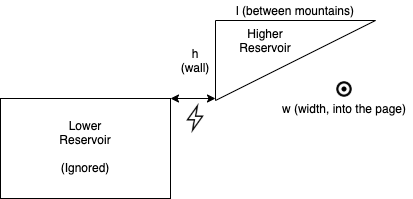
\includegraphics{schema_hydro}
	\caption[Quick schema of the pumped storage station]{Quick schema of the pumped storage station.}
	\labfig{schema_hydro}
\end{marginfigure}


\begin{remark}
Recall that to obtain the energy stored in our hypothetical facility, we simply have to use basic physics.

If $m$ is the mass of water in the reservoir, $g$ the gravitational acceleration constant and $h$ the height of the reservoir, then the potential energy stored in our reservoir is given by~\ref{potential_energy}\footnote{Mind the units!}.

\begin{equation}\label{potential_energy}
E = mgh
\end{equation}

For a 500 meters high wall, and the 2 cubic kilometer reservoir discussed in our hypothetical facility, we have a potential energy of

\begin{equation}\label{potential_energy}
E = 2 \times 10^9 * 1000 * 10 * 500 = 1 \times 10^{16} J = 2.8 TWh
\end{equation}

Note that we multiply by 1000 to get the number of kilograms in our volume of water in cubic meters.

For a 300 meters high wall, the reservoir is now decreased to 1 cubic kilometer, say 1.2 cubic kilometer to account for the simplified geometry. This gives us 1 TWh.

\begin{equation}\label{potential_energy}
E = 1.2 \times 10^9 * 1000 * 10 * 300 = 1 TWh
\end{equation}

\end{remark}

To give a reference, the tallest dam in the world is 300 meters high. To meet the energy storage requirements of a France electricity grid in a 100\% renewable scenario, four of the giant dams should be built. And note that you need to find the location for it.

You can easily see that we are talking about an almost unimaginable scale. The largest dams in the world today would have to become among the smallest\sidenote[][-2mm]{There is a reason the tallest dam in the World, Itaipu Dam, is considered one of the seven wonders of the modern world}.

\begin{itemize}
\item Could every countries build one of these hypothetical facilities?
\end{itemize}

Some will say that it has been done before, so sure. But a lot of countries simply do not have favorable terrain.


\begin{itemize}
\item Could every countries build the necessary multiple infrastructure of this magnitude to meet their storage needs?
\end{itemize}

It is getting difficult to answer with nuance already. If it was the only goal of humanity, this could happen, I guess\ldots


\begin{itemize}
\item Could countries build all the world-record-breaking dams (along with the logistic of flooding valleys somehow) in less than a decade or two?
\end{itemize}

This one is a bit easier to answer. No.


Another things to keep in mind here is the sheer amount of concrete that would be necessary. The financial costs\sidenote[][-2mm]{An enterprise of this magnitude would profoundly change the markets} and, most importantly the energetic costs alone form a physical barrier that I personally cannot conceive being realistically overcome. The Three Gorges dam in China used 28 million cubic meters of concrete. At 700 kWh per cubic meters of concrete, we are talking about around 20 TWh of energy needed to build that structure simply for the concrete. And recall, we need several of those types of dams. It is also worth noting that the impact of concrete manufacturing on $\mathrm{CO_2}$ emissions is not negligible.

%(https://www.grida.no/resources/5404)

Appendix: gravity towers



\section{Materials I -- Lithium and Lead}

Let us consider batteries storage capacity now. We have seen in \refch{renewable_solution} what the batteries needs were for full-renewable scenarios for various countries.

Now, let us look at what this means in terms of feasibility. Batteries require materials, and it happens that the most used materials right now\sidenote[][-2mm]{And the main contributors to the falling costs} are Lithium-Ion batteries and Lead-Acid batteries. Both require, respectively and without surprise, Lithium and Lead, which are mined today. 

\begin{kaobox}[frametitle=The Most Important Question]
We have seen that the costs involved were a problem in and of themselves. But this does not mean this cannot be done, as it has been argued that it might not be that negative of an economic impact due to various, unpredictable factors. This begs the follow-up question:

\begin{itemize}
\item What is the scale of raw materials needed?
\end{itemize}

\end{kaobox}

We will first consider a simple world where Lithium-Ion batteries dominates the market due to prices, as seen today.

We have seen that on a first order, the USA alone would need to install at minima around 30TWh of energy storage capacity to transition its \emph{electric grid only} to a 100\% renewable scenario.

One needs around 130g of Lithium for each kWh delivered by a Li-Ion battery, or in other words, 0.13 MT of Lithium per TWh. Then, we can obtain the total amount of Lithium to be mined in order to install the battery systems needed\sidenote[][-2mm]{Once! Recall that the lifetime of a Li-Ion battery is between 10 to 15 years, which means that you need to mine new materials every time you want to replace your battery}. We see that in the case of the USA electric grid transition, one needs around 4 megatons of Lithium every 10 or so years. Over a century, this means close to 40 megatons. 

Here is the catch. The current proven reserves of Lithium in the world are estimated to be around 70MT.

This means that for the USA electrical grid only, I stress this, over 50\% of the total world reserve are needed. Keeping in mind that we want to transition the total energy production, and not only the electricity, that a few countries would want the Lithium for their own grids, and that Lithium is necessary in a lot of other devices today, we can easily see that this is not sustainable\sidenote[][-2mm]{Not to mention that I really doubt the costs of Lithium would not skyrocket given a supply scarcity, putting a full stop to the "Batteries will get cheaper" argument}.

Another interesting thing to note is that Lithium is not homogeneously distributed in the world, as shown on \vreffig{lithium_reserves_world}~\sidecite{kesler2012global}. Most of the reserves come from South America, and from mines that China recently invested a lot to buy out. This is not my field, but I would not be surprised if this caused some very strong political tensions in the near future.


\begin{figure*}[h]
	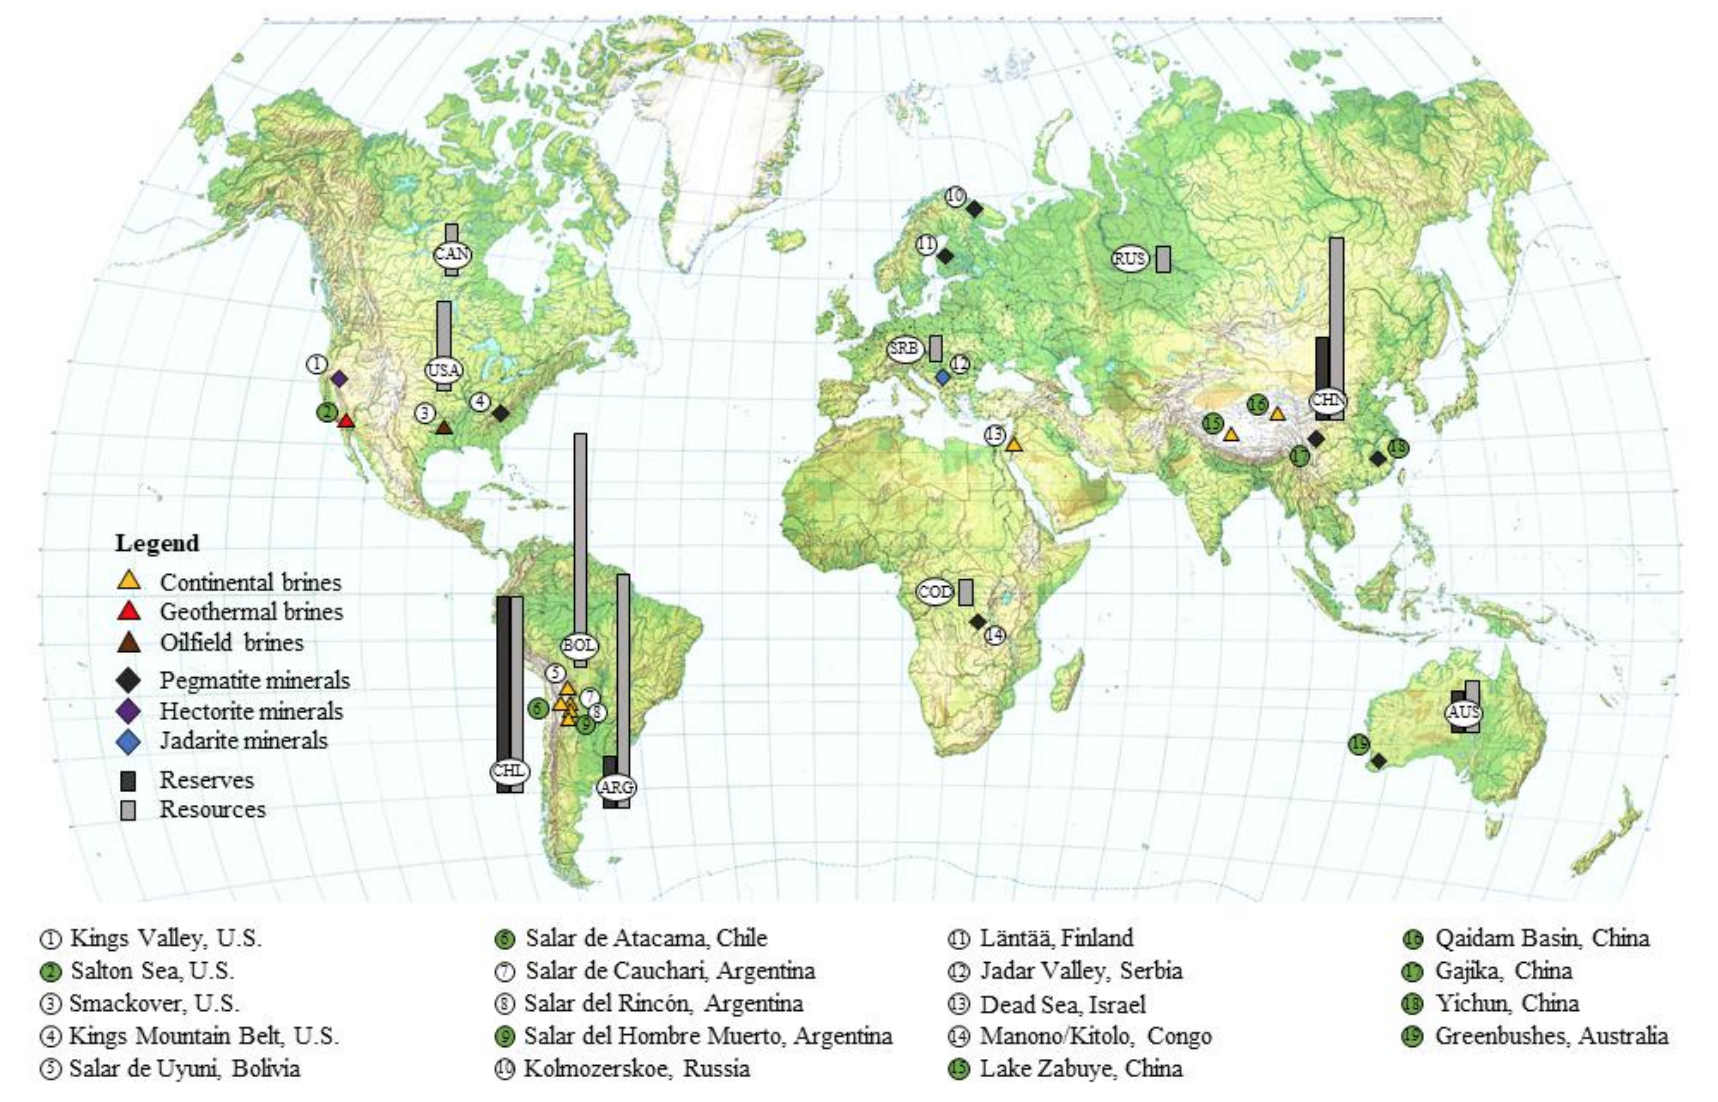
\includegraphics[width=1.0\textwidth]{lithium_reserves_world}
	\caption[Location of selected Li deposits and geographical distribution of global reserves and resources. Green colored labels are sites
known or believed to be currently producing.]{Location of selected Li deposits and geographical distribution of global reserves and resources. Green colored labels are sites known or believed to be currently producing.}
	\labfig{lithium_reserves_world}
\end{figure*}

Let us take a look at the Lead-Acid batteries now, and do a similar assessment of their scaling potential. A Lead-Acid battery contains around 15 kg of Lead per kWh produced. Again, for the USA electrical grid transition, this amounts to 450 MT of Lead every 10 or so years, and 4,500 MT of Lead over the century.

Now, to the catch again. The proven resources of Lead in the world are around 80 MT, and the undiscovered resources estimated at around 2,000 MT. This is an obvious problem, as it is by far lower than the USA requirements to transition their grid alone.

Something to keep in mind in all this is that recycling is an option. Today, it is well developed for Lead, with around 50\% potentially recovered, putting the proven reserves at approximately 50\% more, up to 3,000 MT undiscovered. The recycling process for Lithium is more complex and is still under development\sidenote[][-2mm]{And considering the plastic recycling economy, I find it personally unlikely that this would make great strides necessary to have a scaling effect}. 

\section{Materials II -- Rare Earth Materials}


We saw the problem of Lithium and Lead. You may also have heard of the Rare Earth Elements problem.

\begin{kaobox}[frametitle=Rare Earth Materials]

Rare Earth Elements consists of seventeen metals, most of which are absolutely critical in numerous modern technologies. Yet they are difficult to extract from the crust.

Neodymium and Dysprosium are notably used extensively in wind turbine technology.

\end{kaobox}

We have estimated reserves of 8 MT of Neodymium and 1.5MT of Dysprosium in the world today. Wind power uses approximately 180 kg of Neodymium and 30 kg of Dysprosium per MW.

This implies that the hard limit on installed wind power is around 45,000 GW or 45 TW\sidenote[][-2mm]{This is ignoring the numerous other critical uses of Dysprosium and Neodymium}.

The installed wind power capacity necessary to power the entire US energy sector using wind would be around 8 TW. Given the lifetime of the wind turbine, this puts us at around 30 TW over a century. Obviously, in reality the need would be lower as the grid is not going to be powered by 100\% wind. But it does go to show that in a energy mix of say 50/50 between solar and wind, not even considering the batteries issues we discussed, the world decarbonized energy needs would likely be causing consequential resource issues from Neodynium and Dysprosium notably.

Will we develop a more efficient, more sustainable technology along the way? Maybe. But there is absolutely no guarantees of this\sidenote[][-2mm]{There have been, and still are, strong motivations to avoid the use of Rare Earth Elements, if only due to geopolitical reasons: most of the more easily accessible resources are in China. They have yet to come to something scalable.}.

This is something essential to have in mind when thinking about a sustainable clean energy infrastructure, and another hint at the best solution, a complete mix of low-carbon sources.

\section{Materials III -- Copper}

We can see the pattern here, the finite material problem is the crux of the renewable world, and the technology world in general. Another material of vital importance in the manufacturing of wind turbines, solar panels, and batteries\sidenote[][-2mm]{On top of plethora of essential everyday items} is copper. The reason it is so prevalent is because of its great efficiency at conducting electricity.

Solar energy uses approximately 5,000 tons of copper per GW installed, while wind power uses 2,000 tons of copper per GW installed. Recall from the previous section that switching the entire grid to wind energy would require around 30 TW over a century. This represents 60 megatons of copper, only for the USA. Considering solar energy requires even more, it is safe to assume that this would be close to a lower bound.

The identified reserves are 2100 MT, with an estimated 3600 MT that are undiscovered. The current annual demand for copper represents around 25 MT and accelerating quickly (0.5-1MT additional demand per year). 

\begin{lstlisting}[caption={An example of an incorrect interpolation.}]
year = 0
copper_consumption = 0  # MT
copper_reserves_estimated = 5700 # MT
rate_yearly_change = 0.5  # MT
while i < copper_reserves_estimated:
    copper_consumption += 25 * (1 + j*rate_yearly_change)
    year += 1
print(year)
\end{lstlisting}

Running this little code snippet shows that we can expect, under this rate increase and a business as usual scenario, that we would have around 30 years worth of reserves (identified and undiscovered).

We have discussed previously the danger of extrapolating into the future, and this is exactly what happened here. We took the rate of consumption increase and projected that ad infinitum. This is not a correct assumption, as it is obvious to see that the market would very quickly respond negatively to such a demand. In our case, with our simple first order approach, all we can really say is, well, nothing without a huge uncertainty range.

If we consider that demand stays constant, which is actually a fair, optimistic lower bound in today's digital world, then we see that we could get over two centuries of copper.

$\textrm{Years to depletion} = \frac{5700 \textrm{ (reserves)}}{25 \textrm{ (constant consumption)}} = 228 \textrm{ (years)}$

Or, another way to look at it is to consider what we are likely to use for our existing needs during the next century.

$5700\textrm{ (reserves) } - 100\textrm{ (years) } * 25\textrm{ (consumption) } = 3200\textrm{ (reserves left)}$

We can quickly identify that in this scenario, we will have consumed all the identified resources, and be left with the undiscovered resources\sidenote[][-2mm]{And they could be anywhere}, even before considering a real 100\% renewable worldwide push. Still, it is not unreasonable to assume that these resources can be discovered.

This seems pretty high. Now, let's apply a quick and dirty estimate of the world energy need in installed renewable capacity. The current energy consumption in the world is estimated at around 160000 TWh, or 160 PetaWh. From that let us compute the lower and higher bound of copper consumption from the energy transition to 100\% renewable.

Translating to wind power\sidenote[][-2mm]{recall that wind power has a lower copper usage than solar, and a higher capacity factor, so this would form a lower bound}, and assuming an average capacity factor of 30\%, we compute a needed installed capacity of around 60 TW. Given our time frame of a century for sustainability, we would need to install around 240 TW. At 2 megatons per TW, this brings us to 480 MT.

On the other hand, translating to solar power and assuming an average capacity factor of 20\%, we compute a needed installed capacity of around 
90 TW, or around 365 TW over a century. At 5 megatons per TW, this brings us to 1830 MT.

What we consequently see is that under a very favorable projected consumption rate, considered constant, the needs for Copper over the next century under a 100\% renewable scenario\sidenote[][-2mm]{Without accounting for batteries} can be grossly estimated between 3,000 and 4,300 megatons, or 52\% to 75\% of all undiscovered reserves, and 1.4 to 2 times the discovered resources.

\section{Materials IV -- Platinum}

Platinum is currently vital to any efficient process of producing hydrogen. In a renewable scenario, this would be extremely beneficial to store energy, and create a clean energy economy.

Let us try to estimate the needs for Platinum, and the limitations it would impose on the scale of a hydrogen economy.

https://www.advancedsciencenews.com/is-there-enough-platinum-to-run-a-solar-powered-hydrogen-economy/

\section{Locations I -- Renewable Siting}

\blindtext

\section{Health Production Impact}

Solar panel manufacturing and intensive mining does cause a lot of problems today. This would need to be monitored for such a large extension. Note that his argument applies across multiple domains and is not in any way limited to renewable energy. The scale of the projects makes it that this becomes an important concern to at least be aware of.

\blindtext



\section{The Digest}

\begin{kaoboxgreen}[frametitle=Main Takeaways]

\begin{itemize}
\item The \emph{finite materials problem} is very real and is an unmovable wall in the way of 100\% renewable scenarios.
\item Renewable energy is indeed renewable by definition, but capturing that energy is not renewable.
\item Building up energy storage systems or wind turbines use up either finite geographical locations or finite materials resources at an alarming and absolutely not sustainable rate.
\item Recycling will have to become prevalent for some materials. It will not be enough to cover the needs of a 100\% renewable system, but still absolutely needs to be developed.
\end{itemize}
  
\end{kaoboxgreen}
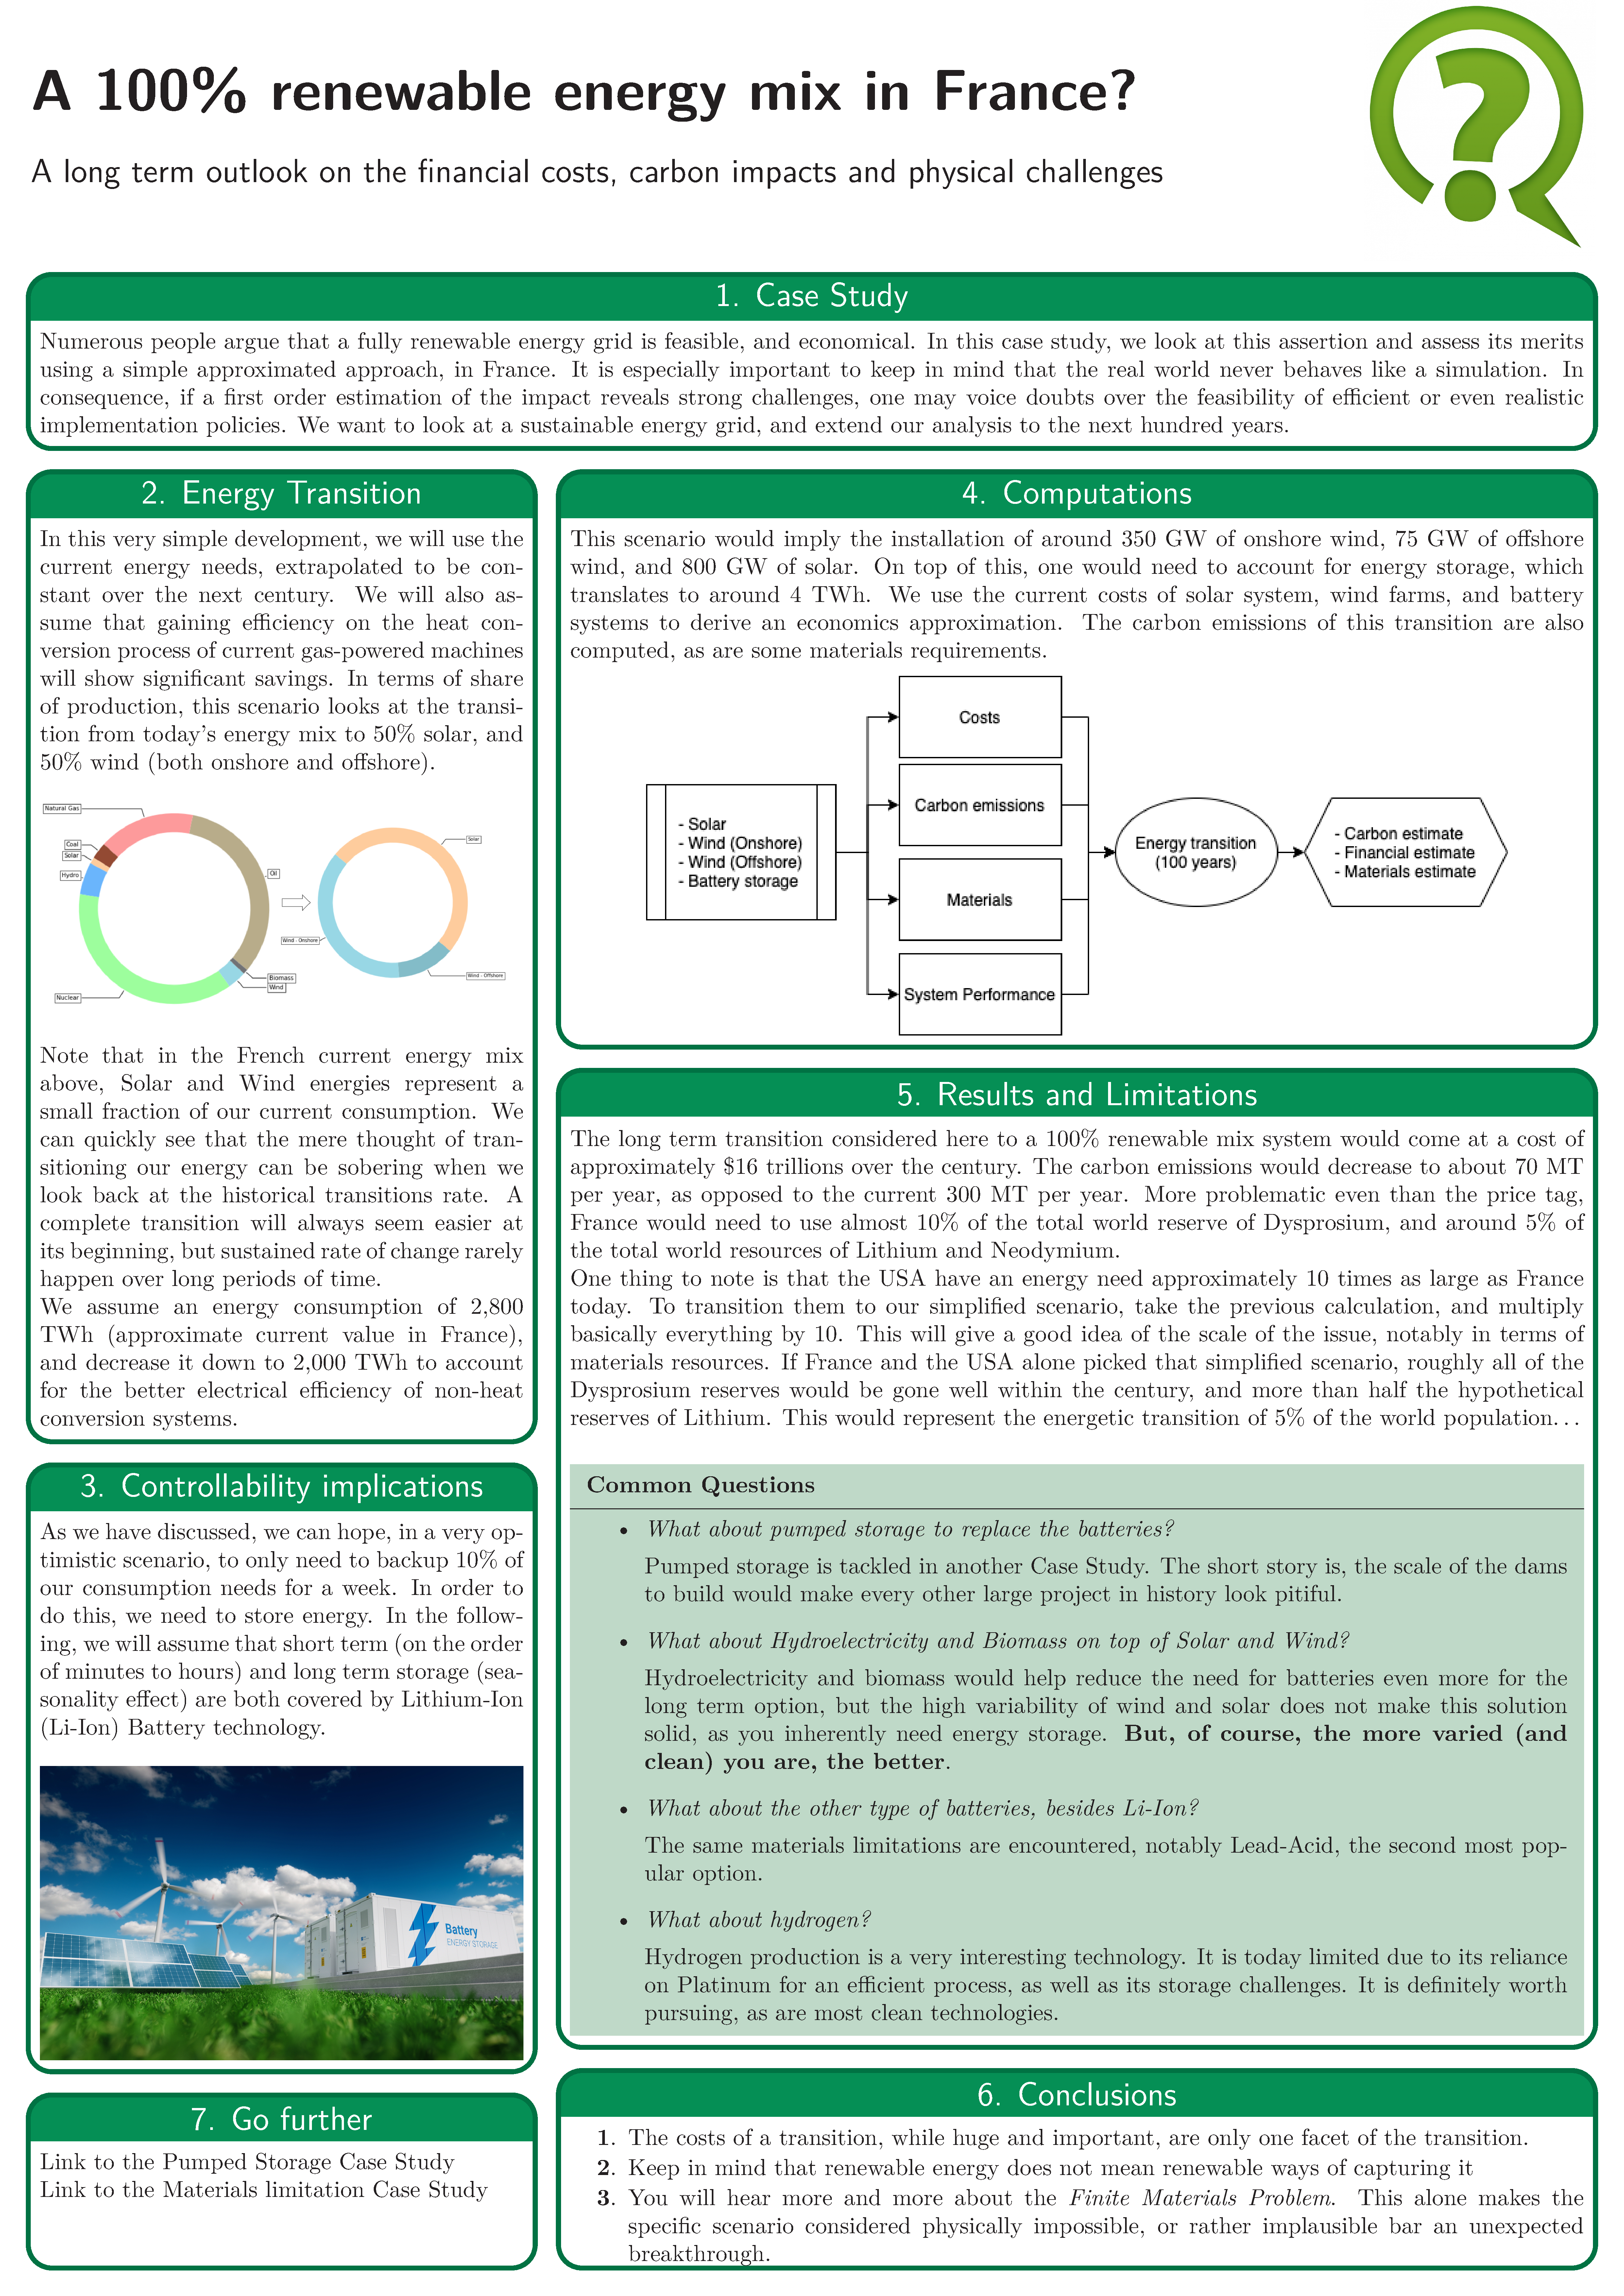
\includepdf[pages=-,addtotoc={1,addsec,1,{Factsheet I -- A 100\% Renewable Energy Mix in France?},test}]{posters/poster_s2a.pdf}
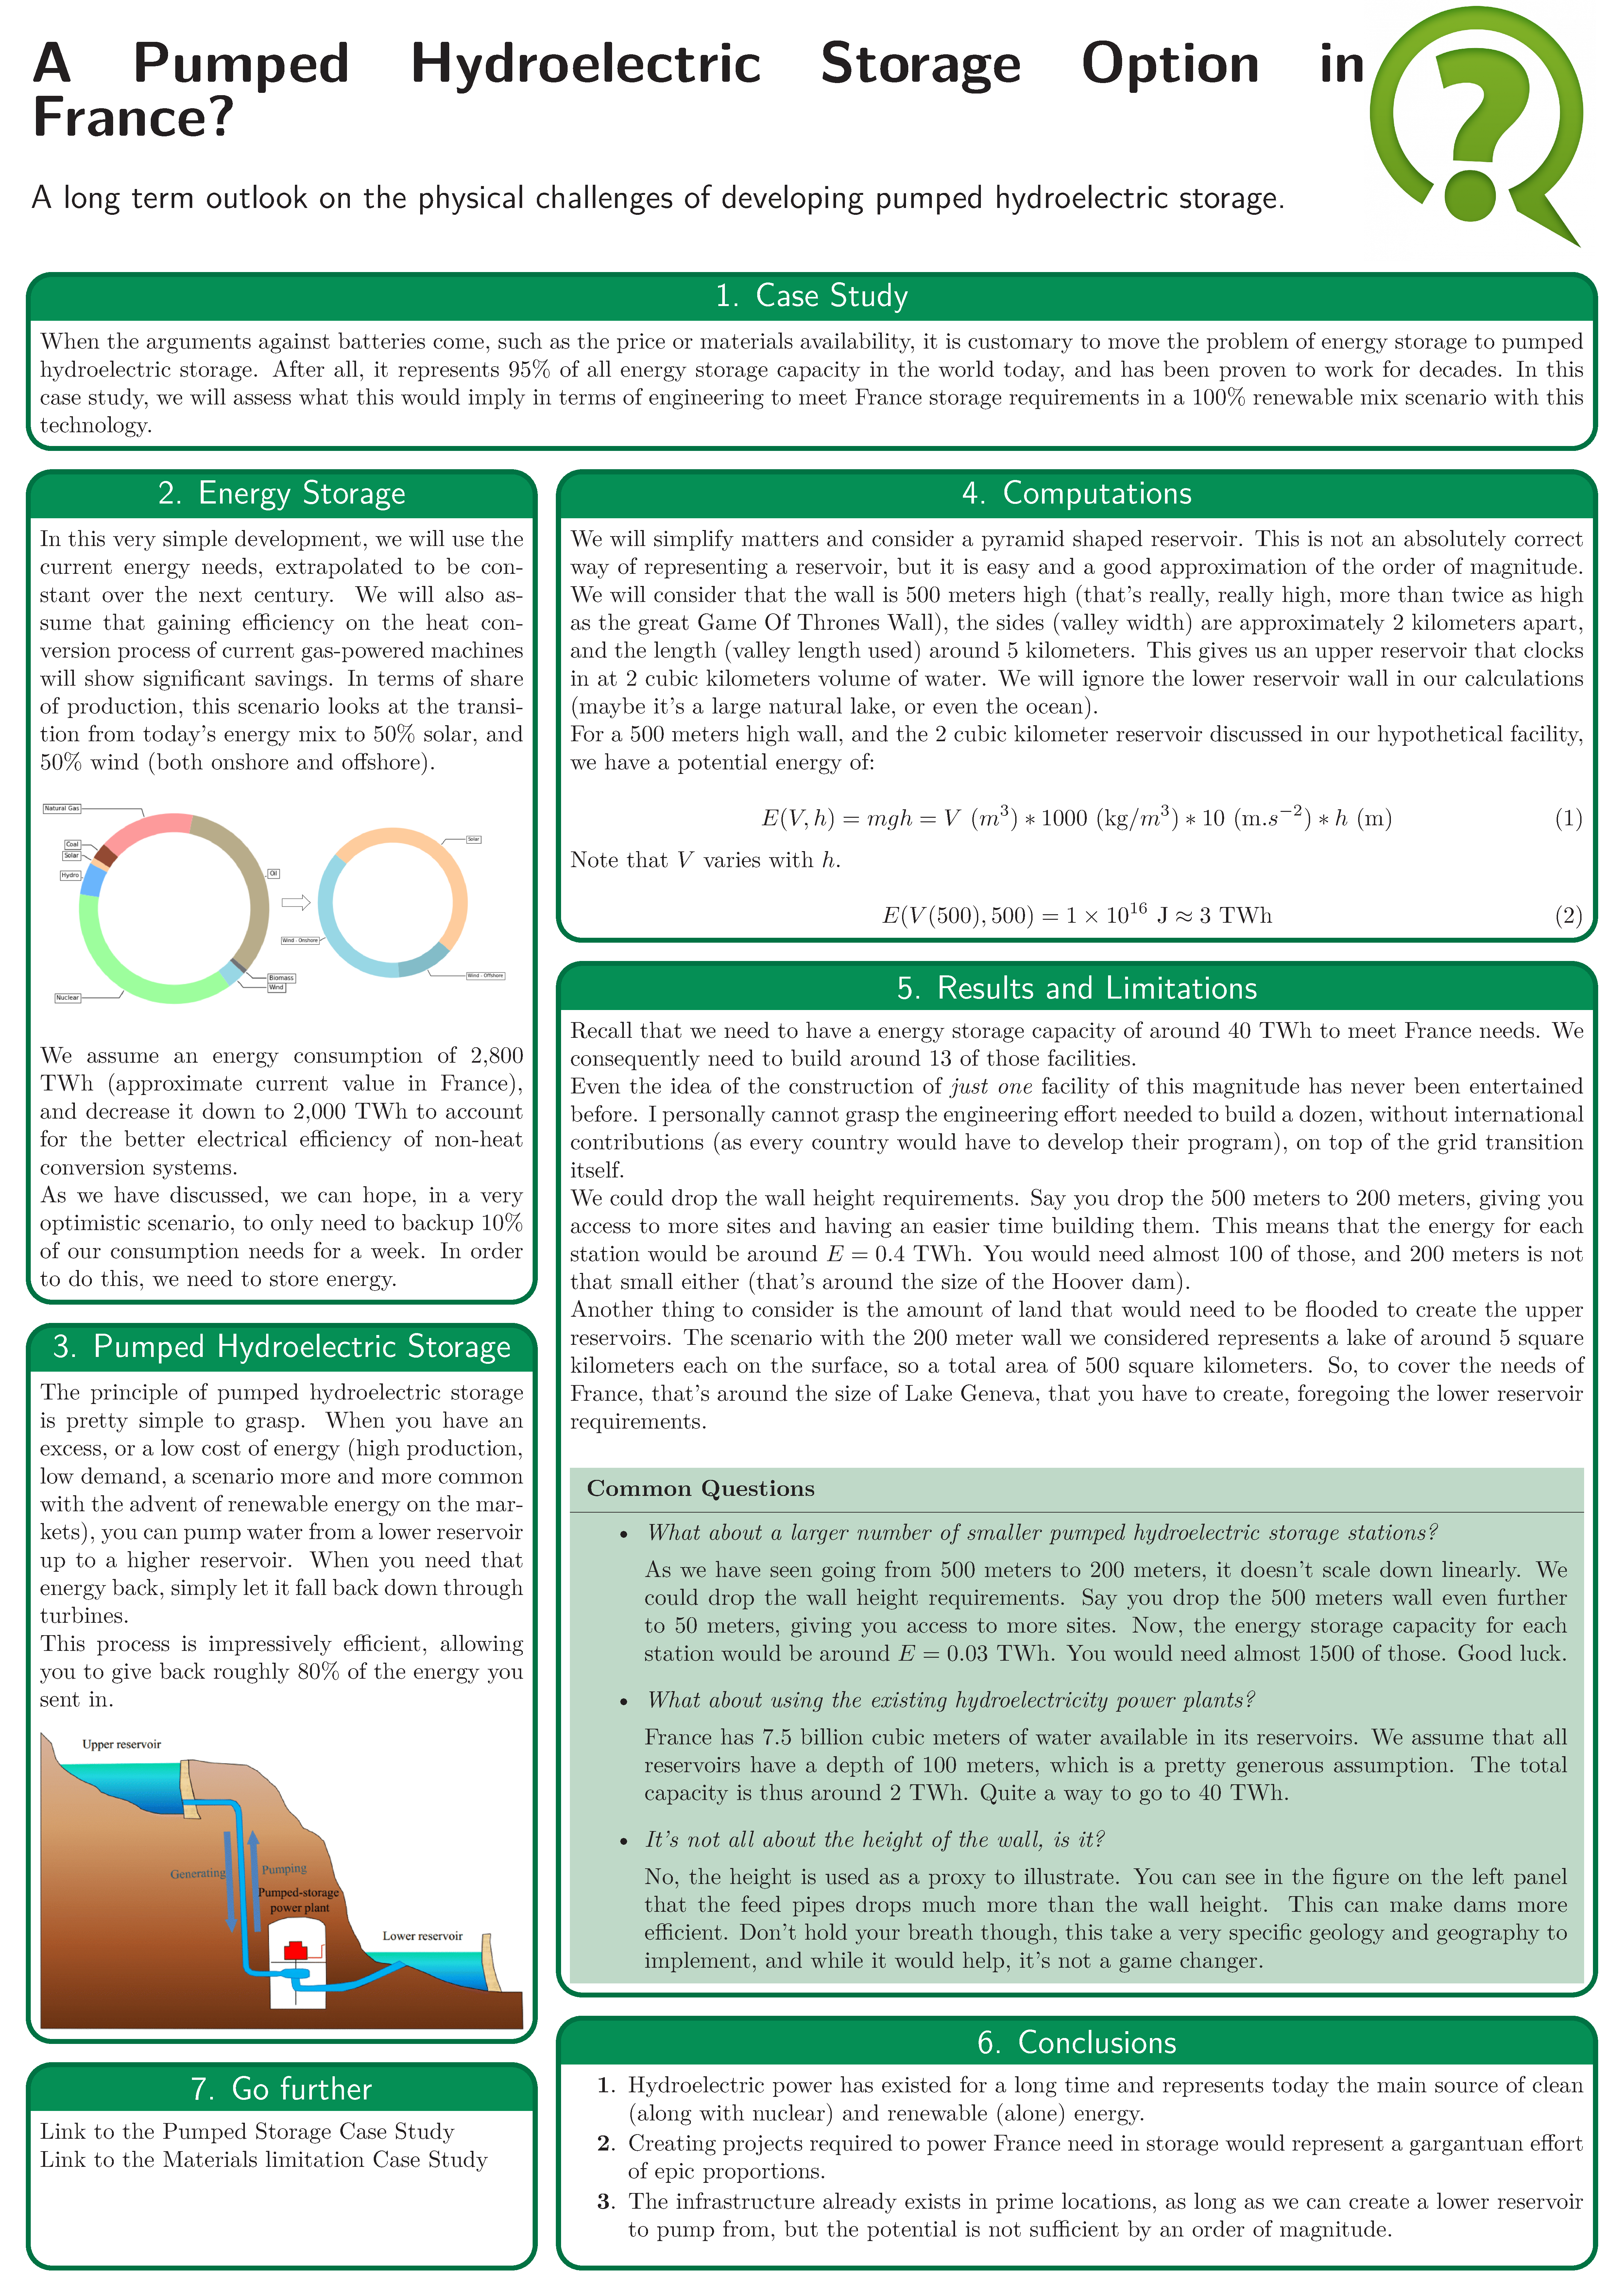
\includepdf[pages=-,addtotoc={1,addsec,1,{Factsheet II -- A Pumped Hydroelectric Storage Option in France?},test}]{posters/poster_pumped_storage.pdf}
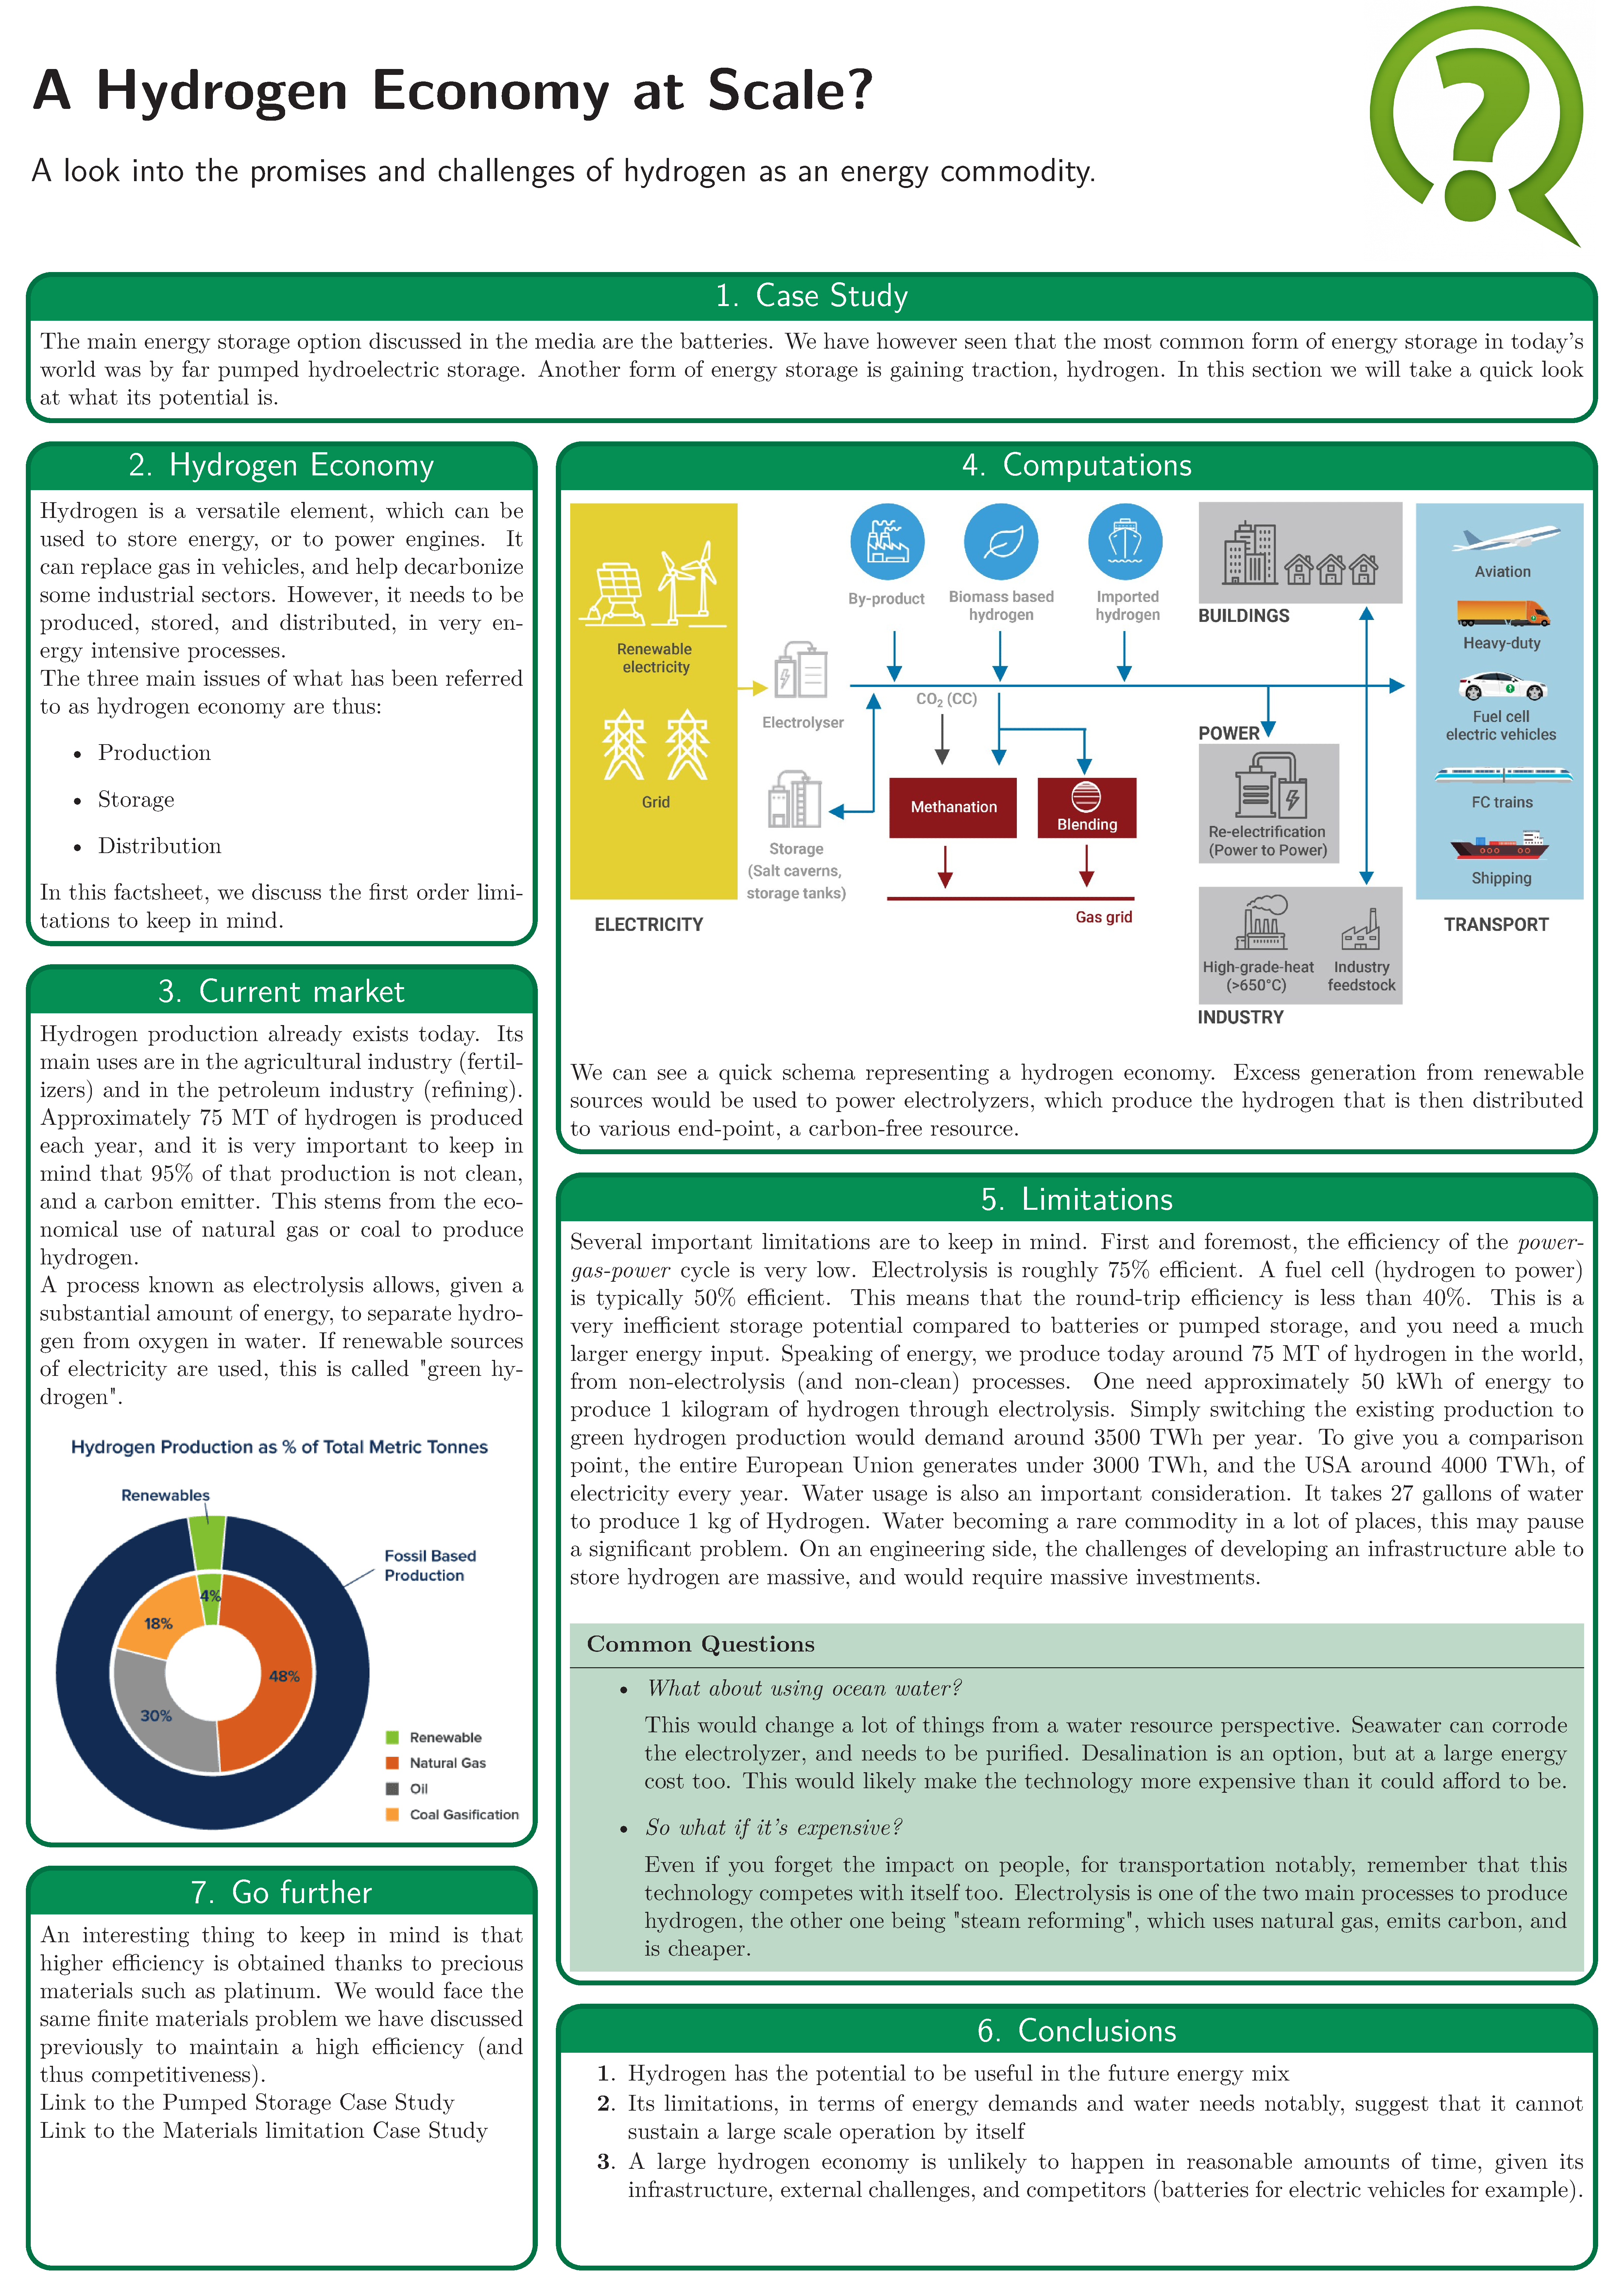
\includepdf[pages=-,addtotoc={1,addsec,1,{Factsheet III -- A Hydrogen Economy at Scale?},test}]{posters/poster_hydrogen.pdf}
\setchapterpreamble[u]{\margintoc}
\chapter{Scenario Assessments -- Nuclear}
\labch{scenario_assessments}

In this chapter I will go over the physical limitations of 100\% Renewable scenarios, from pumped storage locations and scale to batteries materials mining and photovoltaic and wind land area constraints.

This section discusses the issues for nuclear, and for a mix

\section{Locations II -- Nuclear Siting}

\blindtext

\section{Materials V -- Uranium}

Uranium resources are not plentiful despite the punch it can pack~\sidecite{grancea2020uranium}. Available resources are often separated by estimated cost of access, ranging from less than \$40 per kilogram to more than \$260 per kilogram. This gives an estimated reserves between 2.2 and 16 MT.

This severely limits the viability of nuclear on the long term. France alone, going 100\% nuclear for the next century, would need around 2.4 MT.

But, there are silver linings:

\begin{itemize}
\item Fuel recycling: We can, and some countries have had successful recycling programs, which can save up to X\% of the uranium need.
\item Thorium: Nuclear can also work using the Thorium nuclides chain. Thorium is about three times as plentiful as Nuclear.
\item Current reactor technologies use the u-235 isotope of uranium, which occurs at a concentration of 0.7\%. We have since developed advanced reactor which can use natural uranium directly\sidenote[][-2mm]{Several such reactors were tested at scale and even used in actual production, notably in France. They are called breeder because they can transform the 99.7\% fraction of uranium that is $\mathrm{U_238}$ into fissile plutonium, and burn it in a cycle.}.
\end{itemize}

Things are not as simple as simply moving to the advanced reactors however, and it is important to keep that in mind. There are concerns over plutonium proliferation (weapons) in the use of breeder reactors, and there are still many hurdles to overcome to be able to deploy them efficiently at scale.

Removing the recycling ban on nuclear fuel in multiple countries, such as the USA, would go a long way toward buying time.

\blindtext

\section{Public Opinion}

Public opinion is difficult to change quickly and react strongly to fear

\blindtext

\section{Waste}

Waste is an issue, but not a big one. Appendix: Hopes from Oklo

\blindtext

\section{Timeline}

Nuclear takes time to develop, while renewable are fast.

\blindtext

\section{Economical mix}

Renewable need to be super cheap to compete with nuclear fuel generation in today's market, or policies will need to be created to account for this

\blindtext



\section{The Digest}

\begin{kaoboxgreen}[frametitle=Main Takeaways]

\begin{itemize}
\item The \emph{finite materials problem} is very real and is an unmovable wall in the way of 100\% renewable scenarios.
\item Renewable energy is indeed renewable by definition, but capturing that energy is not renewable.
\item Building up energy storage systems or wind turbines use up either finite geographical locations or finite materials resources at an alarming and absolutely not sustainable rate.
\item Recycling will have to become prevalent for some materials. It will not be enough to cover the needs of a 100\% renewable system, but still absolutely needs to be developed.
\end{itemize}
  
\end{kaoboxgreen}
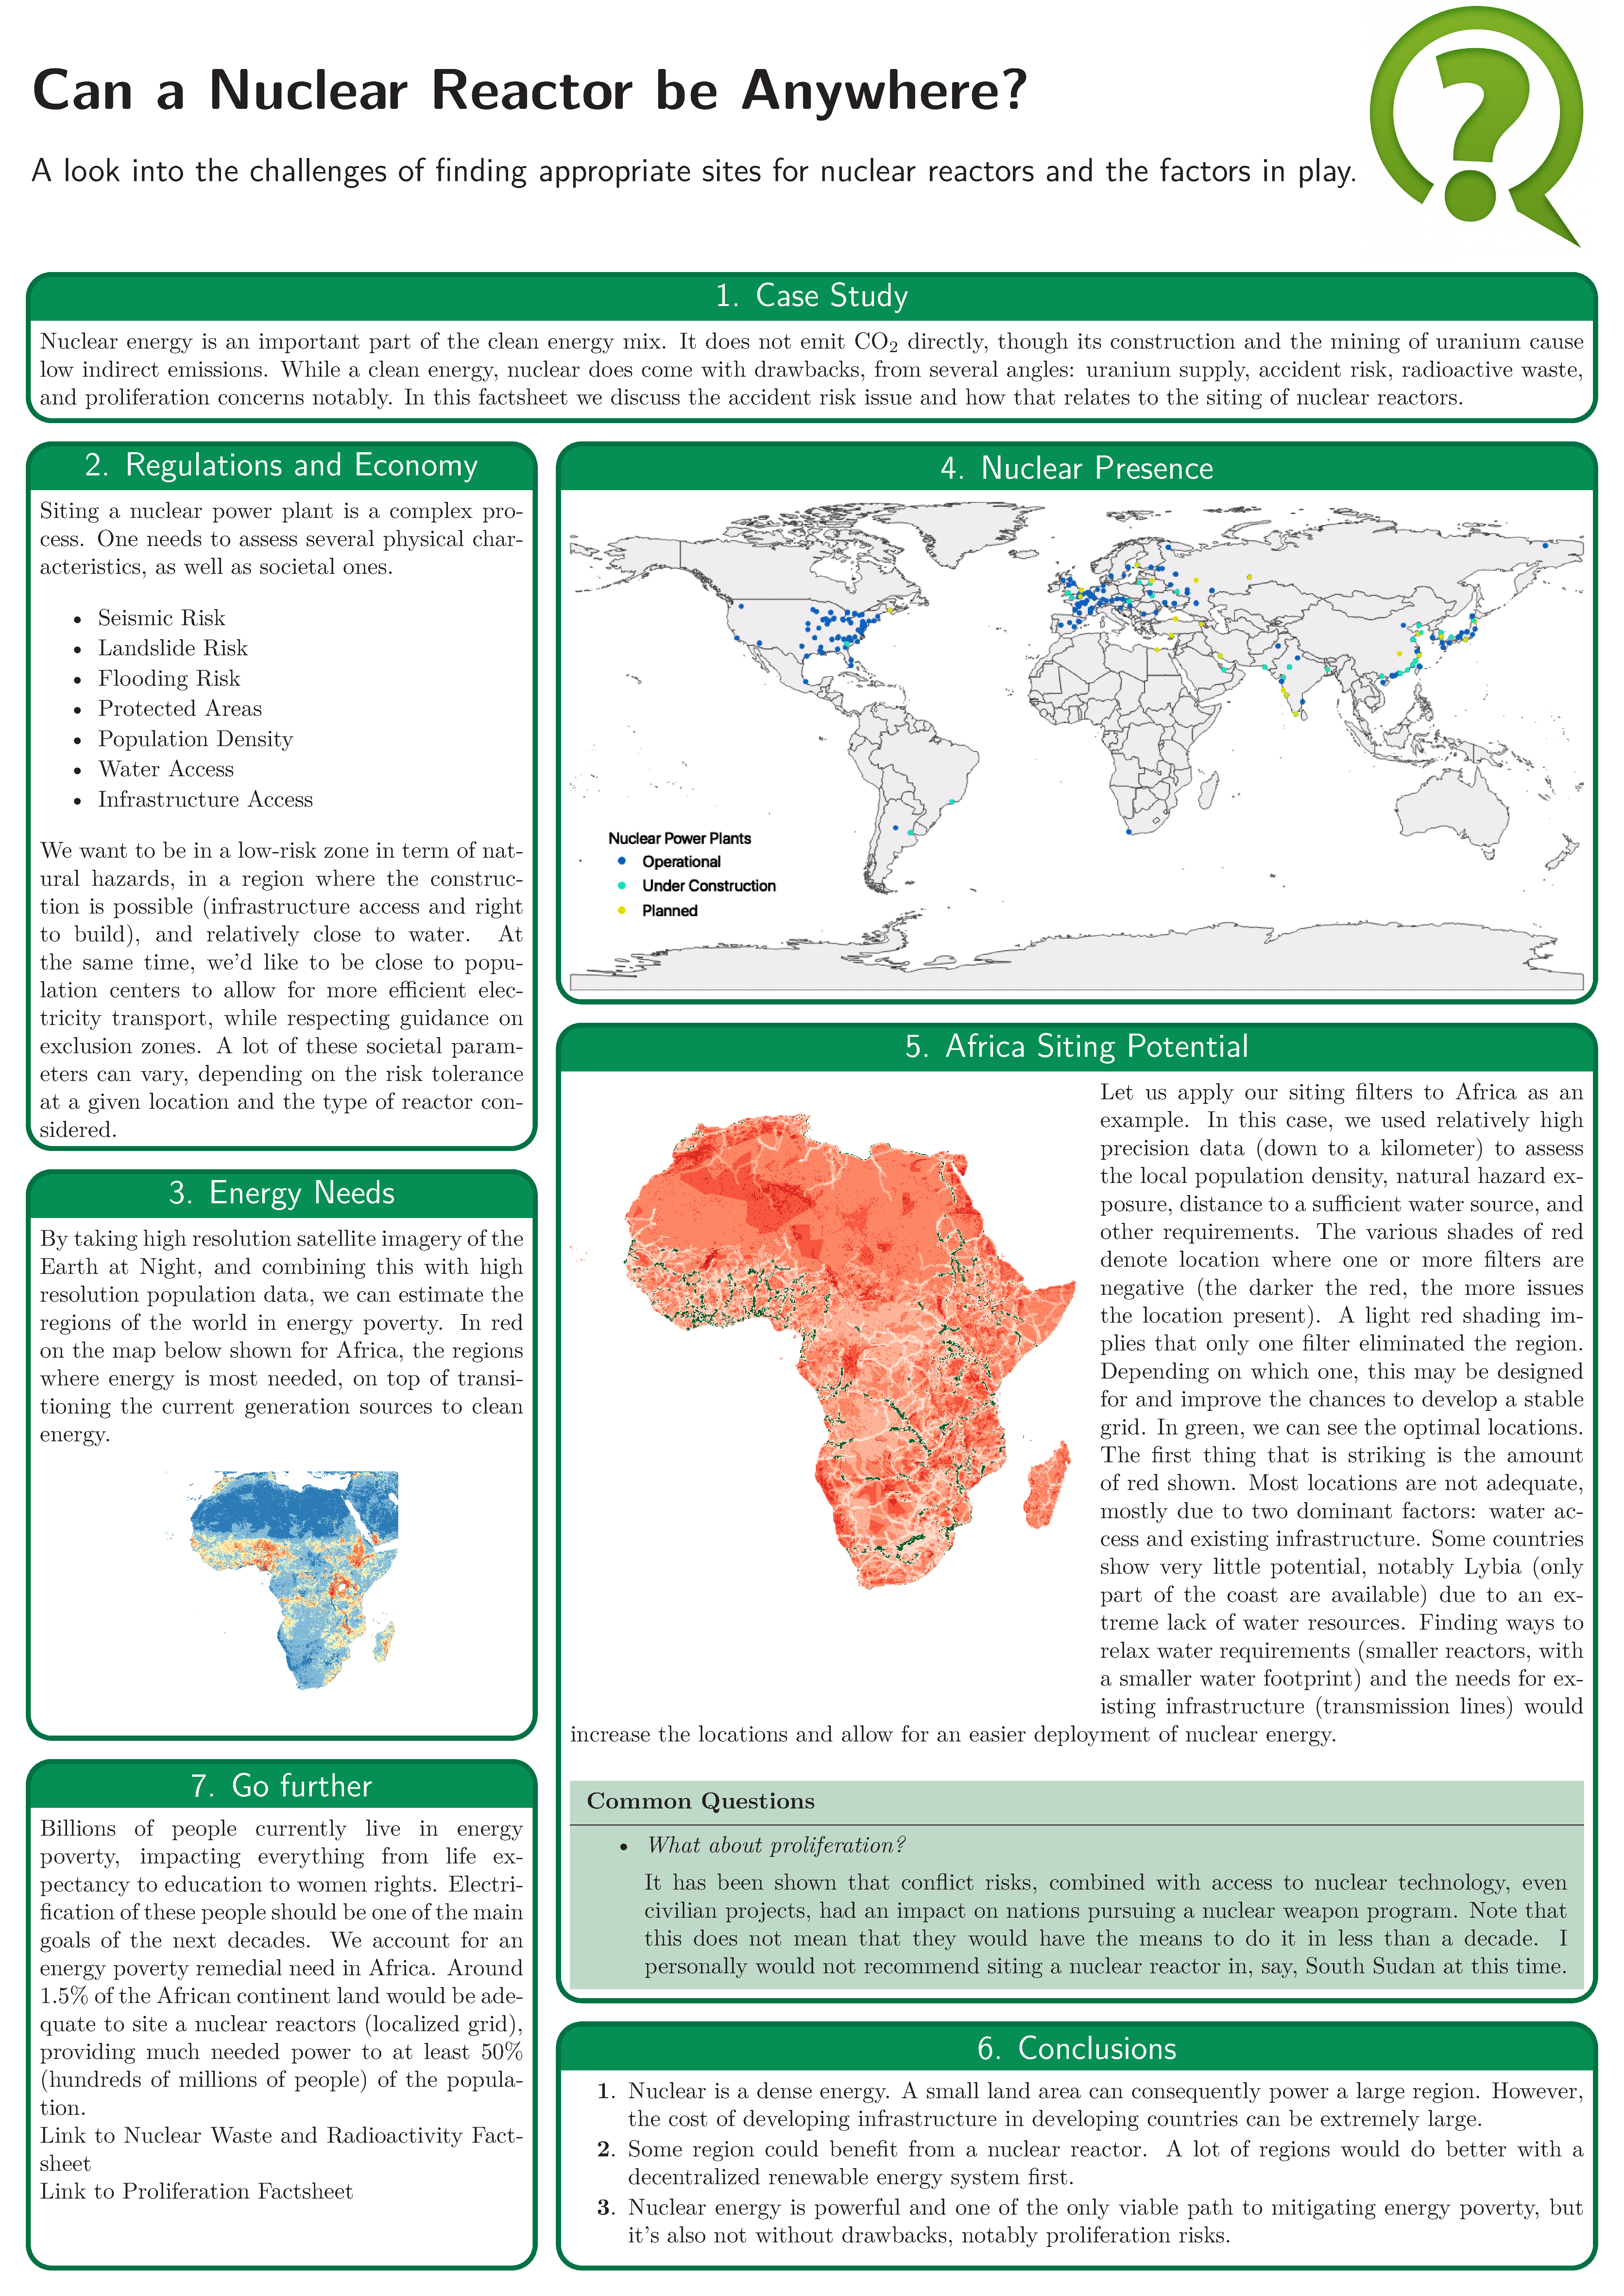
\includepdf[pages=-,addtotoc={1,addsec,1,{Factsheet IV -- Can a Nuclear Reactor be Anywhere?},test}]{posters/poster_nuclear_siting.pdf}
\setchapterpreamble[u]{\margintoc}
\chapter{The Transition Path}
\labch{transition_path}

In this chapter I use the two preceding chapters, on economics, carbon, and issues to draw conclusion on the best, more logical, path forward. I point again that having complex "flux tendu" models that meet the criteria for some countries does not make the problems go away. When the scientific community so strongly disagree, it is wise to err on the side of caution and aim for the least stringent path. If the 100\% renewable camp is wrong and fails to overcome the hurdles, the plan fail. If the "mixed energies, with nuclear" camp is wrong, the plan is still alright. The logical choice is consequently pretty self evident.


\blindtext



\section{Risk Matrix}

We develop a color-coded qualitative risk matrix, with the rows being the scenario, and the columns being the section issue. For example, for S3, nuclear siting is red and uranium is orange, and for S1, copper is orange, RRE is black, Lithium is black, pumped storage is black, etc.

For some technologies, and some materials, the physical limits really seem too large. It is difficult to see how the Dysprosium, Neodymium, Lead or Lithium resource problems could be overcome without a major breakthrough defying the odds. This tends to disqualify batteries system, and consequently severely dampen hopes for a 100\% renewable price, even if the economical impact derived in \vrefsec{renewable_problem} was considered a non-factor.

Copper is likely to become a severe problem over time, though it may not be directly due to the renewable industry. It seems to be within the realm of doable over the next century, even in a full renewable world (though with no batteries, which also use a lot of copper).

A field to seriously explore and develop is the recycling of those materials. Some recycling chains exist currently, at a relatively modest scale. Inherently, with the mines drying up, the cost will go up and make recycling more prevalent\sidenote[][-2mm]{though that also mean a likely cost increase, potentially pricing out some technologies for wide uses}.

\begin{kaobox}[frametitle=TO-DO]
Is there a path around the materials problem? New materials, interesting research, \ldots ?
\end{kaobox}

\section{What does this mean?}

What appears to be the best solution? Is there a choice between multiple scenarios, or is the real, actual, choice only on the share in the mix? Discuss the implications.


\section{The Digest}


\begin{kaoboxgreen}[frametitle=Main Takeaways]

\begin{itemize}
\item This has not been done yet
\item Reading this will teach you absolutely nothing
\item I am serious, I could type random letters and it would give you as much information
\item Fedhiz gavartz hedtz inewps
\end{itemize}
  
\end{kaoboxgreen}

\pagelayout{wide} % No margins
\addpart{A path forward?}
\pagelayout{margin} % Restore margins

\setchapterpreamble[u]{\margintoc}
\chapter{The World Needs}
\labch{world_needs}

In this chapter I scale the renewables scenario to the world, with current assumptions and social assumptions


We are under severe time constraints, and it is important to consider, from what we talked about previously, that continued economic growth is not a fact of nature, and is extremely dependent on energy. Peak oil is approaching quickly, and some countries have passed it already, which notably means that it is likely any energetic transition will have to take place in a recessive context. Investment will not be available in the same way. Conflicts, devastation, migrations on a scale never seen before may also happen due to the climate change very impact, with much stronger hazards, as discussed in a previous section.

We have shown that what is needed, by default of being the only option, is nuclear and renewables, and energy storage for localized use only.

Nuclear “reinstallation” will take time, and we can use that time to ramp up to a good penetration of renewable and make progress. Something is better than nothing, as long as there is a plan.

\blindtext


\section{The Digest}


\begin{kaoboxgreen}[frametitle=Main Takeaways]

\begin{itemize}
\item This has not been done yet
\item Reading this will teach you absolutely nothing
\item I am serious, I could type random letters and it would give you as much information
\item Fedhiz gavartz hedtz inewps
\end{itemize}
  
\end{kaoboxgreen}
\setchapterpreamble[u]{\margintoc}
\chapter{The World is Gone, Long Lives the World}
\labch{not_all_doom}

In this chapter I will go over the fact that it does not have to be all doom and gloom. A net zero is important, but as one can see, the hurdles are immense for the entire world to move toward this. So, does that mean that it is "net zero" or nothing? What does a sufficiently lower emission tally look like in the near future?

Thinking the goal is unattainable is a surefire way of giving up before even trying. In this section, we assess the impact of falling short.

\section{Falling Short}

\blindtext


\section{The Digest}


\begin{kaoboxgreen}[frametitle=Main Takeaways]

\begin{itemize}
\item This has not been done yet
\item Reading this will teach you absolutely nothing
\item I am serious, I could type random letters and it would give you as much information
\item Fedhiz gavartz hedtz inewps
\end{itemize}
  
\end{kaoboxgreen}
\setchapterpreamble[u]{\margintoc}
\chapter{Mental Health -- Coping with the situation}
\labch{mental_health}

In this chapter I mention who we can blame (nobody really), what one can do, what carbon accounting is and how to reasonably use it to better the world.

Fossil fuels replacement is absolutely daunting. Writing off options is the worst thing one can do, it takes a village, and we’ve been on the clock for a while already. But investments need to be made coherently from a unified front.

\begin{itemize}
\item Meditate
\item Vote, with your voice and your wallet
\item Do not go into the fight with a blindfold and one hand behind your back. Nuclear is important.
\item Renewable energies are also important, due to their deployment speed, but do not aim for 100\% renewable, as storage is not a scalable savior and we will get stuck
\item Change your habits, be ready to not be able to watch Netflix at 1am or accept that your electricity may go out at any time.
\end{itemize}



\pagelayout{wide} % No margins
\addpart{Life is Short, this Book is Long\ldots}
%\pagelayout{margin} % Restore margins

\chapter*{If You Have To Remember Something}
\addcontentsline{toc}{chapter}{Summary} % Add the preface to the table of contents as a chapter

This book is long, and it contains a lot of information and calculation estimations. It can be hardy, at times, to sit down and organize all the ideas and insights gained into a useful view of the world and the energy transition.

This section summarizes the main point that tell the story one should care about.

\begin{itemize}
\item Energy is the economy
\item Fossil fuels were an incredible discovery for humanity, but now have us in a technological lock-in, unfortunately too early
\item Climate change will impact us. There is no avoiding it, but we can mitigate its effect by stopping our emissions and increasing our preparedness
\item The scale of the necessary transitions are staggering. Most humans are not very good at three things: thinking at scale,  probability assessment, and complex interlocking networks. Unfortunately, this issue scores high in all three categories.
\item We have the technology to solve most of the issues in theory. Multiple scenarios are possible, and we do have the scientific knowledge to know what can and cannot work.
\item A fully renewable world hits immense hurdles very quickly, because the world has very finite resources.
\item Nuclear is not desirable in a lot of places, because the world is populated with irrational humans.
\item We need to think of a transition in a sustainable way, instead of do the same thing previous generations did: "We did our best, they will have to figure it out". A one-time transition to fully renewable systems may, if the stars align, work. But we do not want to end up stuck with a system that cannot work anymore, the carbon reduction have to be long term.
\item Technological bet is not something I would recommend. Scientists may and will make breakthrough. Their scalability is all that matters, and in that regard media can be misleading.
\item The smartest way, and the best way not to fail, is to go toward a transition mix, where nuclear and renewable are complementary. Location matters.
\item Investing in one technology does not mean not investing in the other. The enemy is carbon-emitting production.
\item We have to stop fighting with one hand in the back, blindfolded, and jumping on one foot.
\end{itemize}


\appendix % From here onwards, chapters are numbered with letters, as is the appendix convention

\pagelayout{wide} % No margins
\addpart{Appendix}
\pagelayout{margin} % Restore margins

\setchapterstyle{lines}
\labch{appendix}
\blinddocument

\chapter{Fonts Testing}

\section{Font Sizes}

{\tiny The quick brown fox jumps over the lazy dog.}

{\scriptsize The quick brown fox jumps over the lazy dog.}

{\footnotesize The quick brown fox jumps over the lazy dog.}

{\small The quick brown fox jumps over the lazy dog.}

{\normalsize The quick brown fox jumps over the lazy dog.}

{\large The quick brown fox jumps over the lazy dog.}

{\Large The quick brown fox jumps over the lazy dog.}

{\LARGE The quick brown fox jumps over the lazy dog.}

{\huge The quick brown fox jumps over the lazy dog.}

{\Huge The quick brown fox jumps over the lazy dog.}


\section{Font Families}

\sffamily\blindtext

\textmd{The quick brown fox jumps over the lazy dog. Medium.}

\textbf{The quick brown fox jumps over the lazy dog. Bold.}

\textup{The quick brown fox jumps over the lazy dog. Upright.}

\textit{The quick brown fox jumps over the lazy dog. Italics.}

\textsl{The quick brown fox jumps over the lazy dog. Slanted.}

\textsc{The quick brown fox jumps over the lazy dog. Small Caps.}

\ttfamily\blindtext

\textmd{The quick brown fox jumps over the lazy dog. Medium.}

\textbf{The quick brown fox jumps over the lazy dog. Bold.}

\textup{The quick brown fox jumps over the lazy dog. Upright.}

\textit{The quick brown fox jumps over the lazy dog. Italics.}

\textsl{The quick brown fox jumps over the lazy dog. Slanted.}

\textsc{The quick brown fox jumps over the lazy dog. Small Caps.}

\rmfamily\blindtext

\textmd{The quick brown fox jumps over the lazy dog. Medium.}

\textbf{The quick brown fox jumps over the lazy dog. Bold.}

\textup{The quick brown fox jumps over the lazy dog. Upright.}

\textit{The quick brown fox jumps over the lazy dog. Italics.}

\textsl{The quick brown fox jumps over the lazy dog. Slanted.}

\textsc{The quick brown fox jumps over the lazy dog. Small Caps.}



%----------------------------------------------------------------------------------------

\backmatter % Denotes the end of the main document content
\setchapterstyle{plain} % Output plain chapters from this point onwards

%----------------------------------------------------------------------------------------
%	BIBLIOGRAPHY
%----------------------------------------------------------------------------------------

% The bibliography needs to be compiled with biber using your LaTeX editor, or on the command line with 'biber main' from the template directory

\defbibnote{bibnote}{Here are the references in citation order.\par\bigskip} % Prepend this text to the bibliography
\printbibliography[heading=bibintoc, title=Bibliography, prenote=bibnote] % Add the bibliography heading to the ToC, set the title of the bibliography and output the bibliography note

%----------------------------------------------------------------------------------------
%	NOMENCLATURE
%----------------------------------------------------------------------------------------

% The nomenclature needs to be compiled on the command line with 'makeindex main.nlo -s nomencl.ist -o main.nls' from the template directory

\nomenclature{$c$}{Speed of light in a vacuum inertial frame}
\nomenclature{$h$}{Planck constant}

\renewcommand{\nomname}{Notation} % Rename the default 'Nomenclature'
\renewcommand{\nompreamble}{The next list describes several symbols that will be later used within the body of the document.} % Prepend this text to the nomenclature

\printnomenclature % Output the nomenclature

%----------------------------------------------------------------------------------------
%	GREEK ALPHABET
% 	Originally from https://gitlab.com/jim.hefferon/linear-algebra
%----------------------------------------------------------------------------------------

\vspace{1cm}

{\usekomafont{chapter}Greek Letters with Pronunciations} \\[2ex]
\begin{center}
	\newcommand{\pronounced}[1]{\hspace*{.2em}\small\textit{#1}}
	\begin{tabular}{l l @{\hspace*{3em}} l l}
		\toprule
		Character & Name & Character & Name \\ 
		\midrule
		$\alpha$ & alpha \pronounced{AL-fuh} & $\nu$ & nu \pronounced{NEW} \\
		$\beta$ & beta \pronounced{BAY-tuh} & $\xi$, $\Xi$ & xi \pronounced{KSIGH} \\ 
		$\gamma$, $\Gamma$ & gamma \pronounced{GAM-muh} & o & omicron \pronounced{OM-uh-CRON} \\
		$\delta$, $\Delta$ & delta \pronounced{DEL-tuh} & $\pi$, $\Pi$ & pi \pronounced{PIE} \\
		$\epsilon$ & epsilon \pronounced{EP-suh-lon} & $\rho$ & rho \pronounced{ROW} \\
		$\zeta$ & zeta \pronounced{ZAY-tuh} & $\sigma$, $\Sigma$ & sigma \pronounced{SIG-muh} \\
		$\eta$ & eta \pronounced{AY-tuh} & $\tau$ & tau \pronounced{TOW (as in cow)} \\
		$\theta$, $\Theta$ & theta \pronounced{THAY-tuh} & $\upsilon$, $\Upsilon$ & upsilon \pronounced{OOP-suh-LON} \\
		$\iota$ & iota \pronounced{eye-OH-tuh} & $\phi$, $\Phi$ & phi \pronounced{FEE, or FI (as in hi)} \\
		$\kappa$ & kappa \pronounced{KAP-uh} & $\chi$ & chi \pronounced{KI (as in hi)} \\
		$\lambda$, $\Lambda$ & lambda \pronounced{LAM-duh} & $\psi$, $\Psi$ & psi \pronounced{SIGH, or PSIGH} \\
		$\mu$ & mu \pronounced{MEW} & $\omega$, $\Omega$ & omega \pronounced{oh-MAY-guh} \\
		\bottomrule
	\end{tabular} \\[1.5ex]
	Capitals shown are the ones that differ from Roman capitals.
\end{center}

%----------------------------------------------------------------------------------------
%	GLOSSARY
%----------------------------------------------------------------------------------------

% The glossary needs to be compiled on the command line with 'makeglossaries main' from the template directory

\setglossarystyle{listgroup} % Set the style of the glossary (see https://en.wikibooks.org/wiki/LaTeX/Glossary for a reference)
\printglossary[title=Special Terms, toctitle=List of Terms] % Output the glossary, 'title' is the chapter heading for the glossary, toctitle is the table of contents heading

%----------------------------------------------------------------------------------------
%	INDEX
%----------------------------------------------------------------------------------------

% The index needs to be compiled on the command line with 'makeindex main' from the template directory

\printindex % Output the index

%----------------------------------------------------------------------------------------
%	BACK COVER
%----------------------------------------------------------------------------------------

% If you have a PDF/image file that you want to use as a back cover, uncomment the following lines

%\clearpage
%\thispagestyle{empty}
%\null%
%\clearpage
%\includepdf{cover-back.pdf}

%----------------------------------------------------------------------------------------

\end{document}
